\chapter{Graph Theory}

\section{Graph Basics}

\begin{definition}
    A \textbf{graph} is a pair $(V,E)$ where $V$ is a finite set, called the \textbf{vertex set}, it's members are called \textbf{vertices}. 
    and $E$ is a collection of subsets of $V$ of size 2. $E$ is called \textbf{edge set}, it's members are called \textbf{edges}.
\end{definition}
\textbf{Remark}:
\begin{itemize}
    \item We generally reserve the name $G$ for graphs.
    \item The textbook likes to write $xy$ or $yx$ to denote an edge. I like more cumbersome notation $\{x,y\}$.
    \item If $x,y \in V$ and $\{x,y\} \in E$, we say $x$ and $y$ are \textbf{adjacent}.
    \item We will not prove things with graphs, but we will think about graphs.
    $$\text{\underline{Think geometrically but proof rigidly.}}$$
    Recall how we proved the pumping lemma in theory of computation.
\end{itemize}


\begin{definition}
    For $n \geq 1$, we let $\mathbf{K_n}$ denote the \textbf{complete graph} $([n],E)$ where $$E=\{e \subset [n]: |e|=2\}$$
\end{definition}
\begin{figure}[ht]
    \centering
    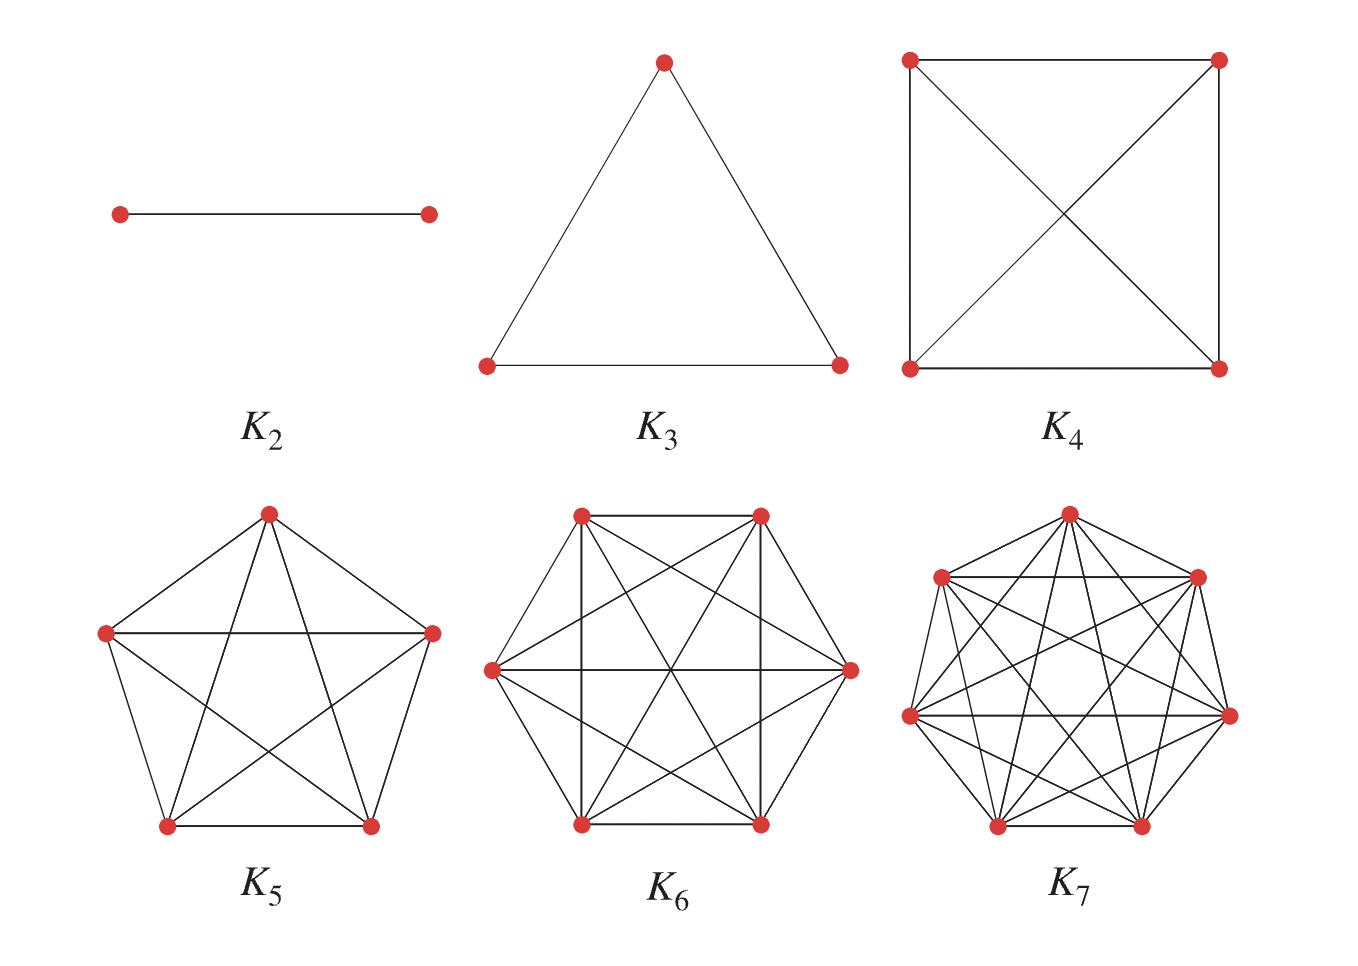
\includegraphics[scale=0.4]{Images/cg.png}
    \caption{A picture of complete graphs}
\end{figure}

\begin{definition}
    For $n \geq 1$, we let $\mathbf{P_n}$ denote the \textbf{path graph}(sometimes called the \textbf{linear graph}) $([n],E)$ where $$E=\{\{i,i+1\} \subset [n]: i \in [n]\}$$
\end{definition}
\begin{figure}[ht]
    \centering
    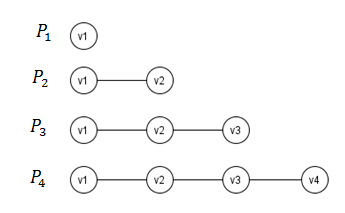
\includegraphics[scale=0.45]{Images/Figure-3Paths-Definition314-The-Cycle-is-a-path-graph-that-its-initial-vertex.jpg}
    \caption{A picture of path graphs}
\end{figure}

\begin{definition}
    For $n \geq 3$, we let $\mathbf{C_n}$ denote the \textbf{cycle graph} $([n],E)$ where $$E=\{\{0,1\},\{1,2\},\cdots,\{n-1,0\}\}$$
\end{definition}
\begin{figure}[ht]
    \centering
    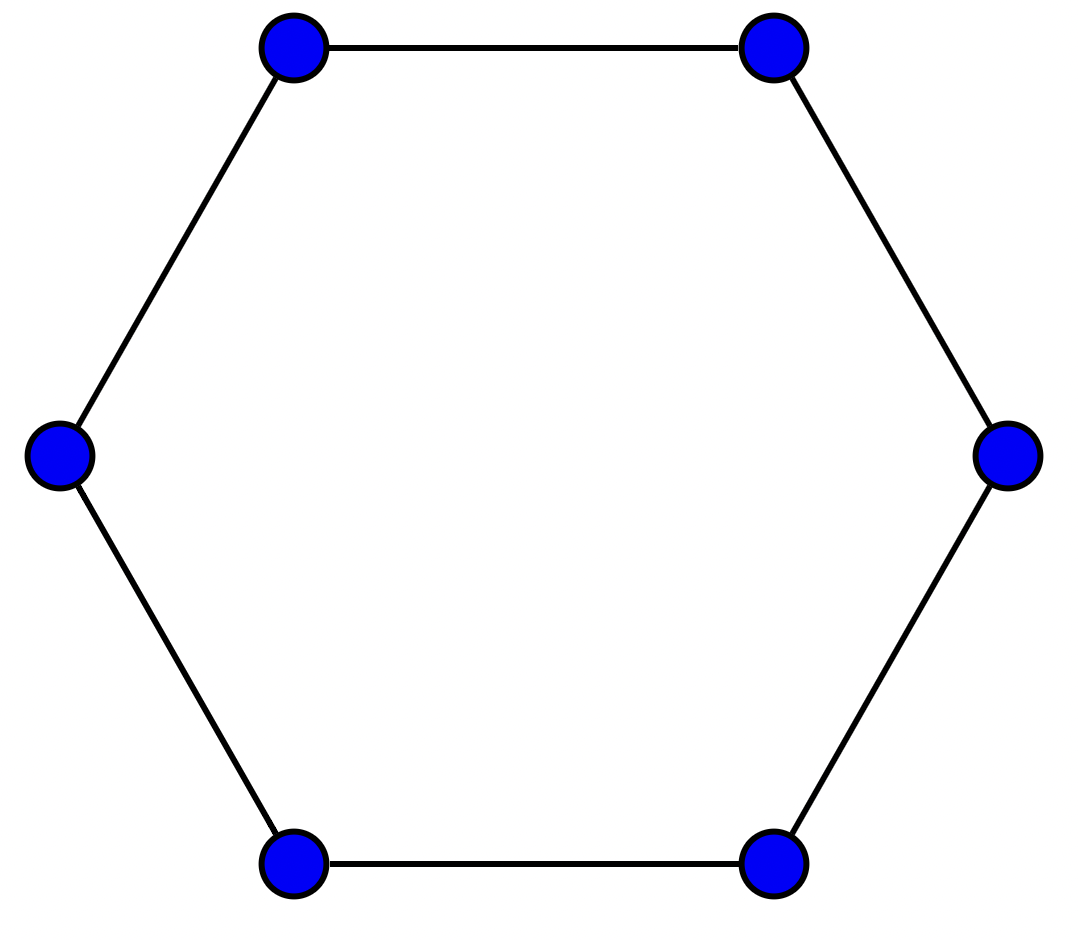
\includegraphics[scale=0.15]{Images/c_6.png}
    \caption{A picture of $C_6$}
\end{figure}

\begin{definition}
    Given a graph $G=(V,E)$, a \textbf{subgraph} of $G$ is a pair $H=(W,E')$ such that $W \subset V$ and $E' \subset \{s \in E: s \subset W\}$. 
    We sometimes abuse notation and write $H \subset G$.
\end{definition}


\begin{definition}
    Given a graph $G=(V,E)$, an \textbf{induced subgraph} is one of the form $$(W,\{\{x,y\} \in E: \{x,y\} \subset W\})$$
    where $W \subset V$
\end{definition}
\begin{figure}[ht]
    \centering
    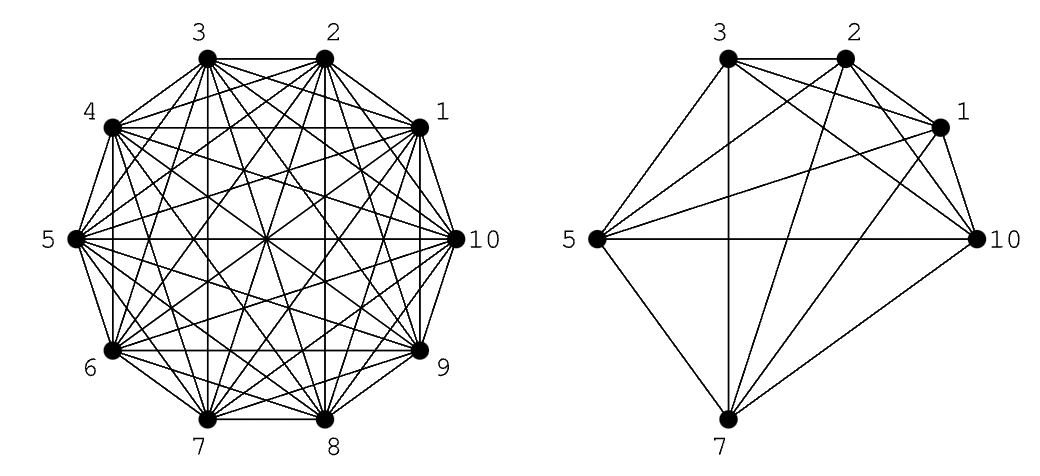
\includegraphics[scale=0.4]{Images/isb.png}
    \caption{A picture of induced subgraph}
\end{figure}
\textbf{Remark}:
\begin{itemize}
    \item Induced subgraphs are uniquely determined by the vertex set, while the standard subgraph is not.
\end{itemize}

\begin{definition}
    Let $G=(V_1,E_1)$ and $H=(V_2,E_2)$ be graphs. 
    We say $G$ and $H$ are \textbf{isomorphism} if there is a bijectiion $$f:V_1 \longrightarrow V_2$$
    with the property that $$\{x,y\} \in E_1 \Longleftrightarrow \{f(x),f(y)\} \in E_2$$
\end{definition}


\begin{theorem}
    Let $G$ be a graph with $n$ vertices. $G$ is isomorphic to a subgraph of $K_n$.
\end{theorem}
\textbf{Remark}:
\begin{itemize}
    \item The above is false if we require the subgraph be induced.
\end{itemize}


\begin{definition}
    Given a graph $G=(V,E)$, and a vertex $v \in V$, we let $$deg_G(v)=|\{u \in V: \{u,v\} \in E\}|$$
    Given a graph $G$, we can create a sequence $(deg_G(v): v \in V)$ of degrees called a \textbf{degree sequence}.
\end{definition}

\begin{theorem}
    Let $G$ and $H$ be graphs, and $f:G \longrightarrow H$ be an isomorphism. 
    Then $$deg_G(x)=deg_{H}(f(v))$$
\end{theorem}


\begin{corollary}
    If $G$ and $H$ have different degree sequences(under any possible ordering), then thsy are not isomorphic.
\end{corollary}

\begin{lemma}[The Handshaking Lemma]
    Let $G=(V,E)$ be a graph, and let $|E|=e$ then $$\sum_{v \in V}deg_G(v)=2e$$
\end{lemma}
\begin{proof}
    For each $v \in V$, let $E_v=\{\{u,v\}:\{u,v\}\in E\}$ denotes all edges around $v$. 
    Notice that for distinct $u,v$, $|E_u \cap E_v| \leq 1$.
    \begin{itemize}
        \item $|E_u \cap E_v| = 1$ when $u,v$ form an edge.
        \item No three distict sets overla.
    \end{itemize}
    It follows that
    \begin{equation}
        \begin{split}
            e &= |E|\\
            &=|\cup_{v \in V}E_v|\\
            &= \sum_{v \in V}|E_v| - \sum_{u,v \in V}|E_u \cap E_v|\\
            &= \sum_{v \in V}def_G(v)-e
        \end{split}
    \end{equation}
    Therfore, $\sum_{v \in V}deg_G(v)=2e$.
\end{proof}


\begin{definition}
    A \textbf{walk} of a graph $G$ is a sequence of vertices $x_1,\cdots,x_n$ that are each successively connected with an edge.
\end{definition}

\begin{definition}
    A \textbf{path} of a graph $G$ is a sequence of \underline{distinct} vertices $x_1,\cdots,x_n$ that are each successively connected with an edge. 
    We call the number of edges in the sequence the \textbf{length of the path}. 
\end{definition}


\begin{definition}
    We call a graph $G$ \textbf{connected} if every part of distinct vertices is connected by a path.
\end{definition}

\begin{definition}
    Given a graph $G$, we denote a maximally connected vertex set a \textbf{connected component}. 
    More formally, if we denote the equivalence relation $\sim$ on $V$ given by $v \sim w \Longleftrightarrow v=w$ or $v$ is connected to $w$. 
    The connected components are the equivalent classes given by this relation.
\end{definition}
\begin{figure}[ht]
    \centering
    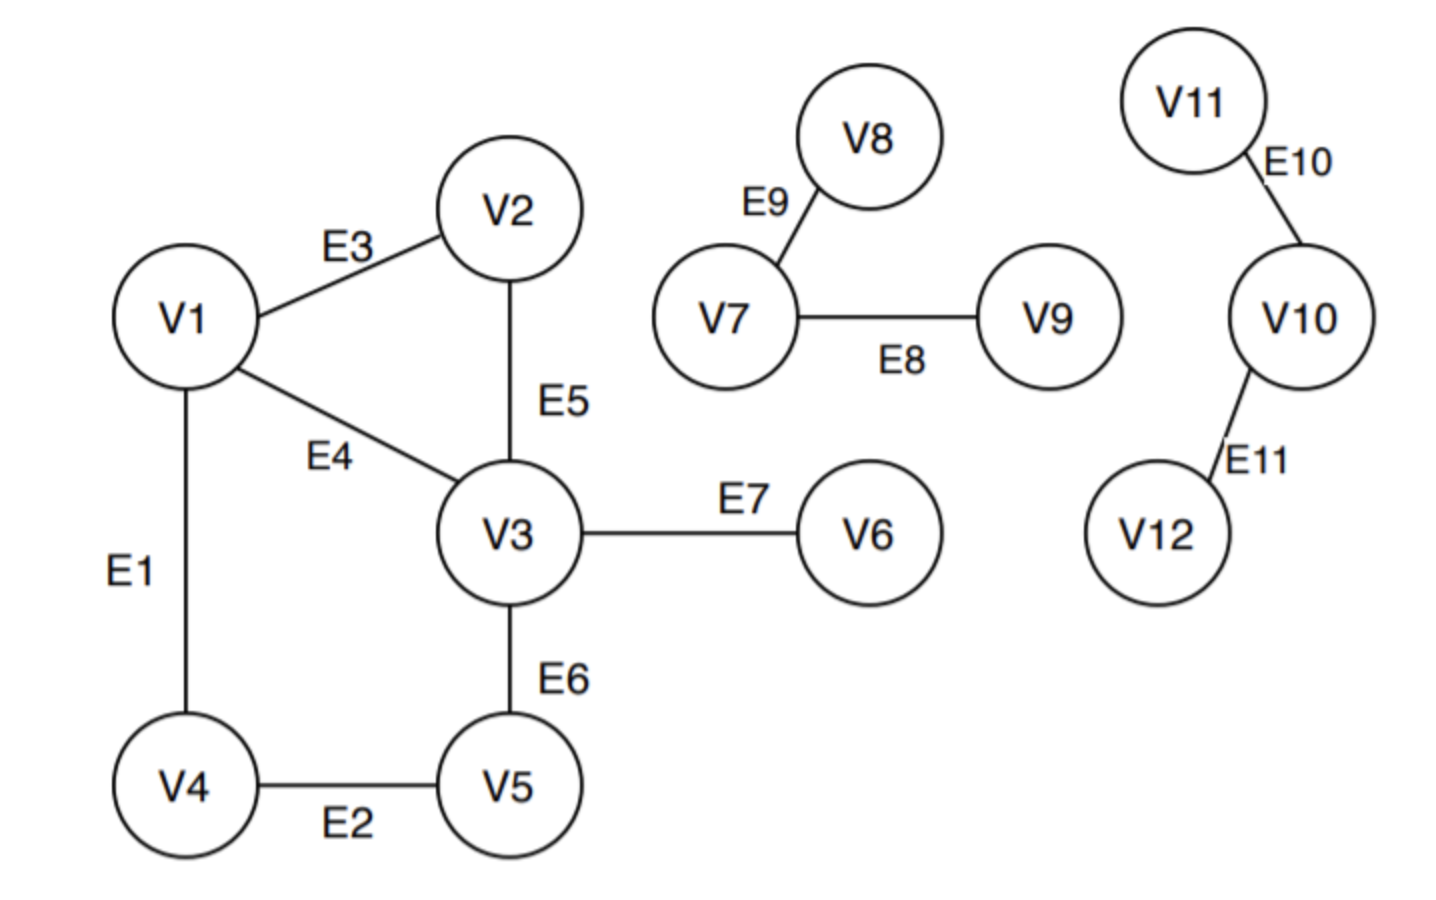
\includegraphics[scale=0.3]{Images/3components.png}
    \caption{A picture of a graph with 3 components}
\end{figure}
\textbf{My Question}:
\begin{itemize}
    \item What is the relation between this and the connected component in topology?
    \item A graph $G$ is a structured set, what is the topology for this set?
\end{itemize}



\section{Trees}

\begin{definition}
    A \textbf{tree} is a graph $G=(V,E)$ with the property that every two vertices are connected by a \underline{unique} path.
\end{definition}
\textbf{Remark}:
\begin{itemize}
    \item The definition implies a tree is connected.
    \item Trees are the minimally connected objects.
\end{itemize}
\begin{figure}[ht]
    \centering
    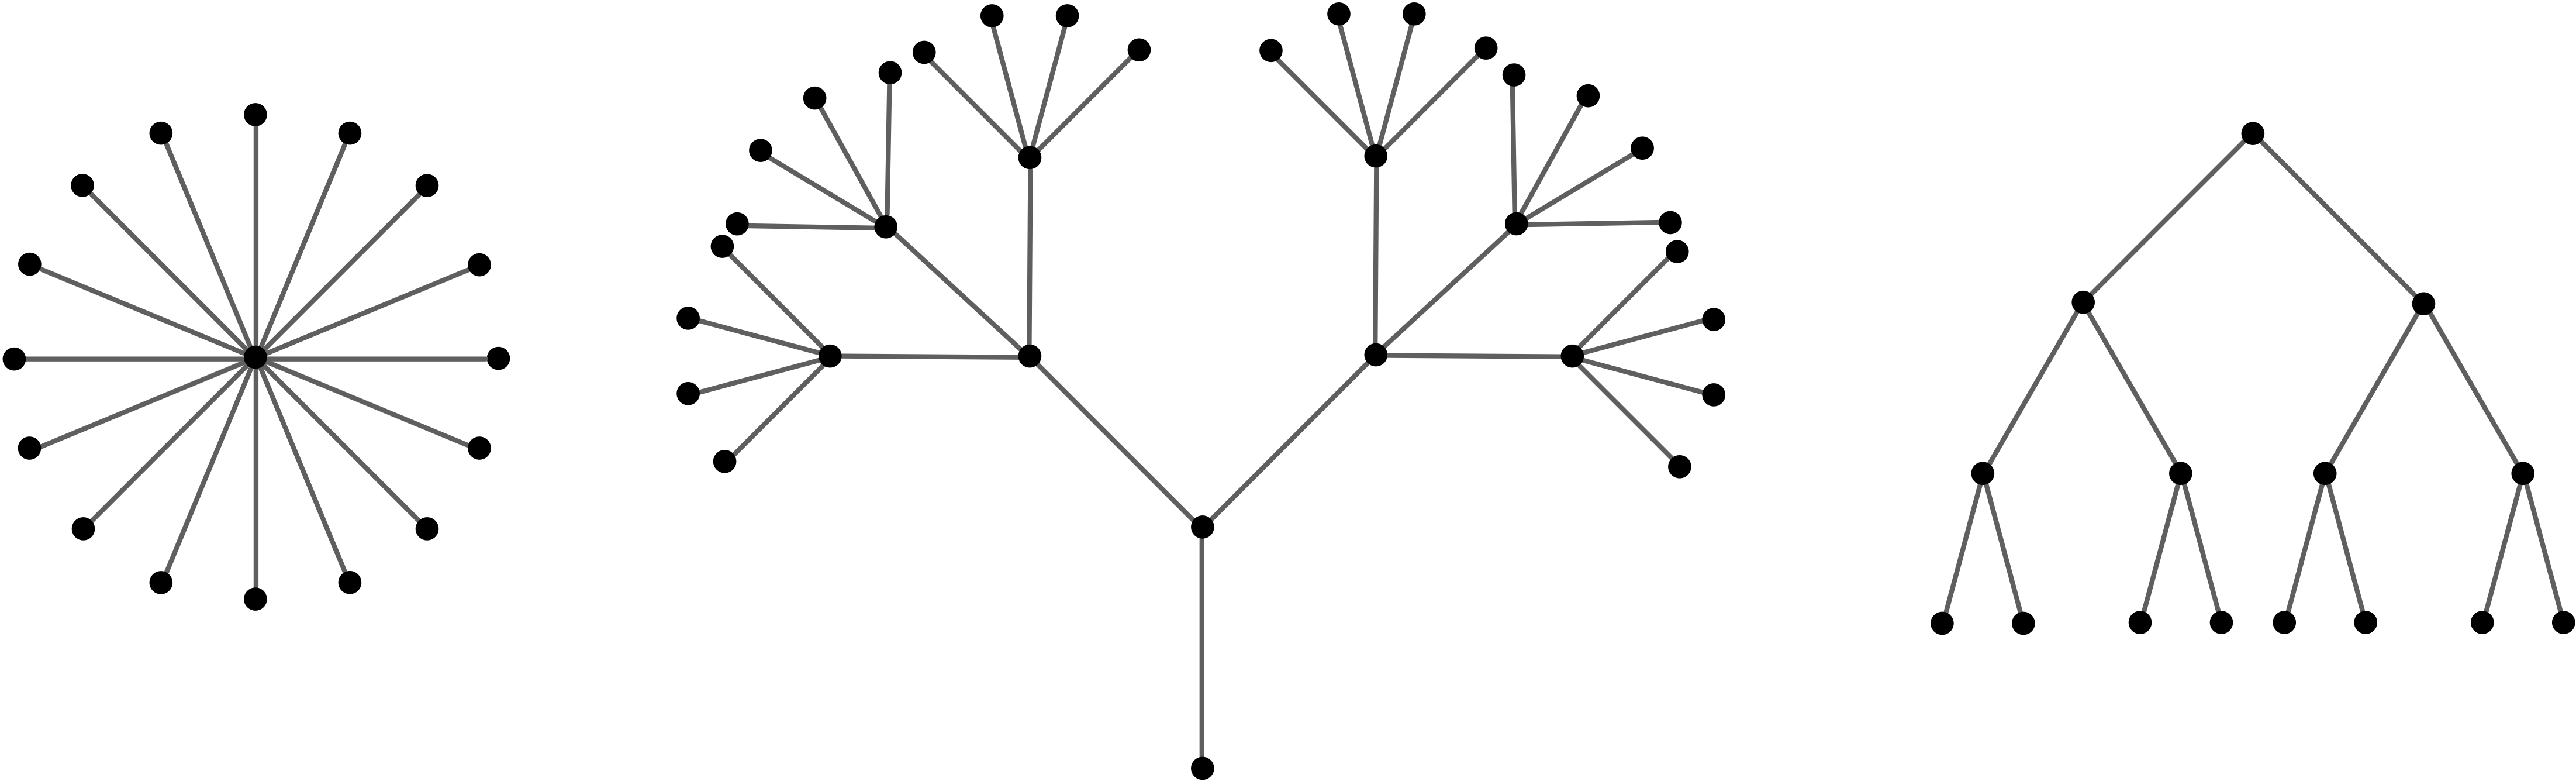
\includegraphics[scale=0.15]{Images/forest.png}
    \caption{A picture of 3 trees}
\end{figure}

In order to prove the next theorem, we need the following lemmas.

\begin{lemma}
    If $G=(V,E)$ is connected and has no cycle, then $$\exists v \in V. deg_V(v)=1$$
    (For any vertex $v$ hs such property will be called a \textbf{leaf}.)
\end{lemma}
\begin{proof}
    (Prove by contradiction.)\\
    Let $G=(V,E)$ be a connected graph with $n$ vertices and has no cycle. Suppose $\forall v \in V. deg_V(v) \geq 2$.
    Consider the procedure:
    \begin{itemize}
        \item Set $i=2$. Select any vertex to be $v_1$, and trace an edge $e_1$ from $v_1$ to some neighboring vertex $v_2$.
        (This is possible because the tree has at least 2 vertices and is connected.)
        \item From $v_i$, trace $e_i \neq e_{i-1}$ to $v_{i+1} \neq v_i$.
        \item Set $i \mapsto i+1$. Repeat from step2.
    \end{itemize}
    \begin{figure}[ht]
        \centering
        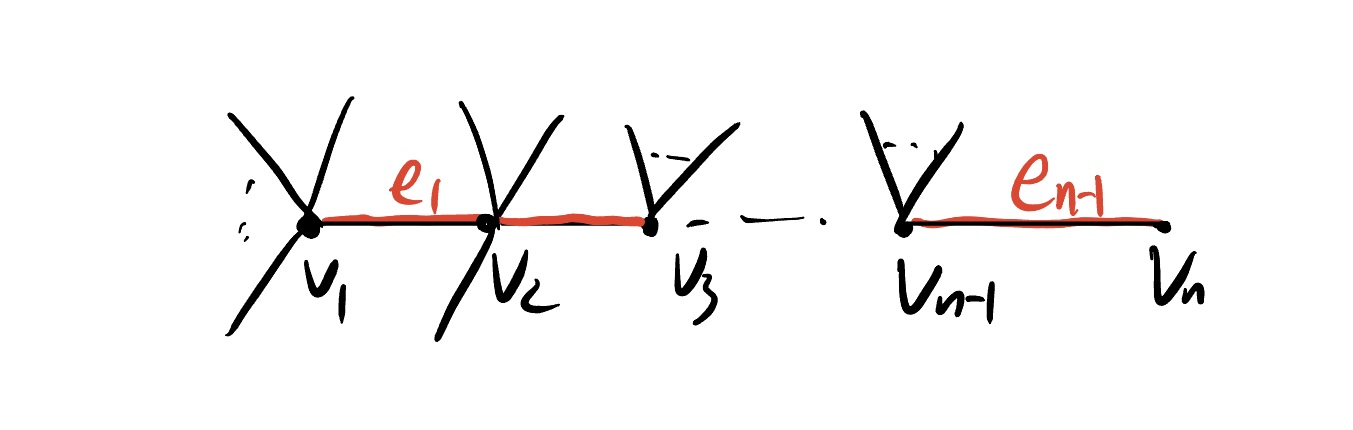
\includegraphics[scale=0.14]{Images/lemma_pic.jpg}
        \caption{A picture of applying the lemma}
    \end{figure}
    Hence for $v_n$, there must be an $e_n$, connecting one of $\{v_1,\cdots,v_{n-1}\}$.\\
    Therefore, we have a cycle. This is a contradiction.
\end{proof}



\begin{lemma}[Characterisation of bridge]
    An edge $e$ of a graph $G$ is a bridge if and only if $e$ lies on no cycle of $G$.
\end{lemma}


\begin{theorem}
    Let $G$ be a connected graph with $n$ vertices. The following are equivalent.
    \begin{enumerate}
        \item $G$ is a tree.
        \item $G$ does not contain a cycle.
        \item $G$ has $n-1$ edges.
    \end{enumerate}
\end{theorem}
\begin{proof}
    We are going to show that
    $$(1) \Longrightarrow (2) \Longrightarrow (3) \Longrightarrow (1)$$
    \begin{enumerate}
        \item Suppose $G$ is a tree. Suppose there is a cycle $x_1,x_2,\cdots,x_n$ with $\{x_i,x_{i+1}\}$ and $\{x_n,x_1\}$. 
        Notice, 
        \begin{itemize}
            \item $x_1,\cdots,x_n$ is a path from $x_1$ to $x_n$.
            \item $x_1,x_n$ is also a path from $x_1$ to $x_n$.
        \end{itemize}
        This contradicts to uniqueness.
        \item Let $n$ be the number of vertices, we are going to do induction on $n$.\\
        Base case:$n=1$, there is 0 edge, true.\\
        Inductive step: Assume $(2) \Longrightarrow (3)$ is true for $n$. 
        Let $G=(V,E)$ be a connected graph with $n+1$ vertices with no cycle. 
        By the first lemma, there exists $v_k$ that has only one edge. 
        Let $\{v_t,v_k\}$ denotes that edge. Remove $v_k$ and $\{v_t,v_k\}$ from $G$. Can show easily that the new graph $G'$ is connected. (Since $\forall v_p,v_q \in V$, there exists a path from $v_p$ to $v_q$ and $v_k$ cannot be in this path, otherwise there will have repetition.)
        By induction hypothesis, $G'$ has $n-2$ edges. Therefore, $G$ has $n-1$ edges.
        \item Do strong induction on number of vertices $n$.\\
        Base case: $n=1$, true.\\
        Inductive step: Assume $(3) \Longrightarrow (1)$ is true for $n$. 
        Let $G$ be a connected graph on $n+1$ vertices with $n$ edges. 
        If $G$ has cycle, then there are at least $n+1$ edges. This is a contradiction, hence $G$ has no cycle. 
        Pick any edge $\{v_p,v_q\}$ from $G$. 
        By the second lemma, $\{v_p,v_q\}$ is a bridge. 
        Remove this bridge, by definition of bridge, we have two connected components. 
        Let us denote them as $G_1=(V_1,E_1),G_2=(V_2,E_2)$, $V=V_1 \coprod V_2$. 
        For any $u,v \in V$
        \begin{itemize}
            \item $u,v$ both in $V_1$ or $V_2$. By induction hypothesis, we are done.
            \item $u,v$ in different connected components. Without loss of generality, assume $u \in V_1,v \in V_2$. 
            By induction hypothesis, there is a unique path from $u$ to $v_p$ in $G_1$, and a unique path from $v_p$ to $v$ in $G_2$. 
            Connected two paths with $\{v_p,v_q\}$, we have a unique path from $u$ to $v$ in $G$.
        \end{itemize}
    \end{enumerate}
\end{proof}


\begin{definition}
    Let $T=(V,E)$ be a tree. We call a vertex $v$ a \textbf{leaf} if $deg_T(v)=1$.
\end{definition}

\begin{lemma}
    Let $T$ be a tree with at least 2 vertices, then $T$ has atleast two leaves.
\end{lemma}

\begin{definition}
    Given a graph $G=(V,E)$, we call a subgraph $H \subset G$ \textbf{spanning} if $H=(V,E')$ where $E' \subset E$.
\end{definition}

\begin{definition}
    Given a graph $G$, a \textbf{spanning tree} is a subgraph $T \subset G$ that is a tree.
\end{definition}

\begin{theorem}
    Every connected graph has a spanning tree.
\end{theorem}

\noindent \textbf{Questions}:Prove:
\begin{itemize}
    \item A graph is connected $\Longleftrightarrow$ it has a spanning tree.
    \item $G$ is a tree $\Longleftrightarrow$ the removal of any edge disconnects $G$.
\end{itemize}

\begin{definition}
    A \textbf{labeled tree} is a tree $T$ whose vertex set is $\{1,\cdots,n\}$.i.e. The vertex set is ordered.
\end{definition}

\begin{definition}[\textbf{Algorithm to convert a Prüfer sequence into a tree}]
    Fix $n \geq 2$, let $s:[n-2] \longrightarrow \{1,\cdots,n\}$ be a sequence.
    ($s$ is a sequence that has length $n-2$ ,every digit is a number from 1 to $n$)
    Consider the following algorithm that generates a set $E$ of size $k-1$
    \begin{itemize}
        \item Find the smallest $j$ which is not in the range of $s$(find the smallest number in$\{1,\cdots,n\}$ that we didn't use.)
        Put $\{j,s(0)\}$ in $E$. Set $L=\{1,\cdots,n\} \setminus \{j\}$ and delete the first entry of the sequence to get a new sequence $s$
        \item Suppose we 're at a stage $i$. Find the smallest $j$ in $L$ that is not in the range sequence. 
        Add $\{j,s(0)\}$ to $E$ (recall $s(0)$ may be different now as we 're truncated $s$). Remove $j$ from $L$ 
        and truncate $s$ by removing the first entry again.
        \item When the string $s$ is empty, $L$ contains two elements. Add $L$ to $E$.
    \end{itemize}
\end{definition}
\textbf{Remark}:
\begin{itemize}
    \item The above assigns each sequence $s$, a set $E$ of size $n-1$, such that the associated graph $(\{1,\cdots,n\},E)$ is connected
\end{itemize}
\begin{figure}[ht]
    \centering
    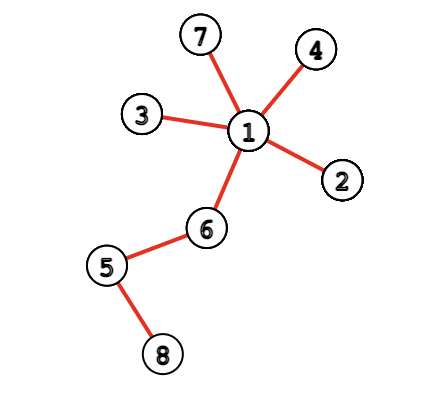
\includegraphics[scale=0.5]{Images/pfc111165.png}
    \caption{Prüfer Code: 111165}
\end{figure}



\begin{definition}[\textbf{Algorithm to convert a tree into a Prüfer sequence}]
    Suppose we have a labeled tree $T=(\{1,\cdots,n\},E)$. 
    We associated to $T$ a sequence $s:[n-2] \longrightarrow \{1,\cdots,n\}$ defined as follows:
    \begin{itemize}
        \item $s(0)$ is the unique vertex adjacent to the leaf witthe smallest indes. Delete this leaf and move to the nest stage.
        \item $s(i)$ is the unique vertex adjacent to the leaf with the smallest index in the new tree gotten from deleting the last leaf.
        \item The process will terminate when the tree becomes a single edge with two leaves.
    \end{itemize}
\end{definition}
\textbf{Remark}:
\begin{itemize}
    \item To each labeled tree, there is a unique Prüfer code associated to it.
\end{itemize}


\begin{theorem}[Cayley]
    For each $n \geq2$, there are exactly $n^{n-2}$ labeled trees on $\{1,\cdots,n\}$
\end{theorem}
\begin{proof}
    To each tree, find the unique associated Prüfer code $s:[n-2] \longrightarrow \{1,\cdots,n\}$. 
    This puts labeled trees in bijective correspondence with sequences $s$. 
    There are exactly $n^{n-2}$ such sequences. Hence exactly many trees. 
\end{proof}


\section{Eulerian Graphs}

\begin{definition}
    Given a graph $G=(V,E)$, an \textbf{Eulerian circuit} is a sequence of vertices $x_0,\cdots,x_t$ with the property that:
    \begin{itemize}
        \item $x_0=x_t$
        \item $\forall i \in [t]. \{x_i,x_{i+1}\} \in E$
        \item $\forall e \in E. \exists i \in [t]. e=\{x_i,x_{i+1}\}$ and this choice is unique. i,e, every edge appears exactly once.
    \end{itemize}
\end{definition}
\textbf{Remark}:
\begin{itemize}
    \item The reason why the Eulerian path came up with, is initially solve the problem: \underline{Bridges of Könisberg}.
\end{itemize}
\begin{figure}[ht]
    \centering
    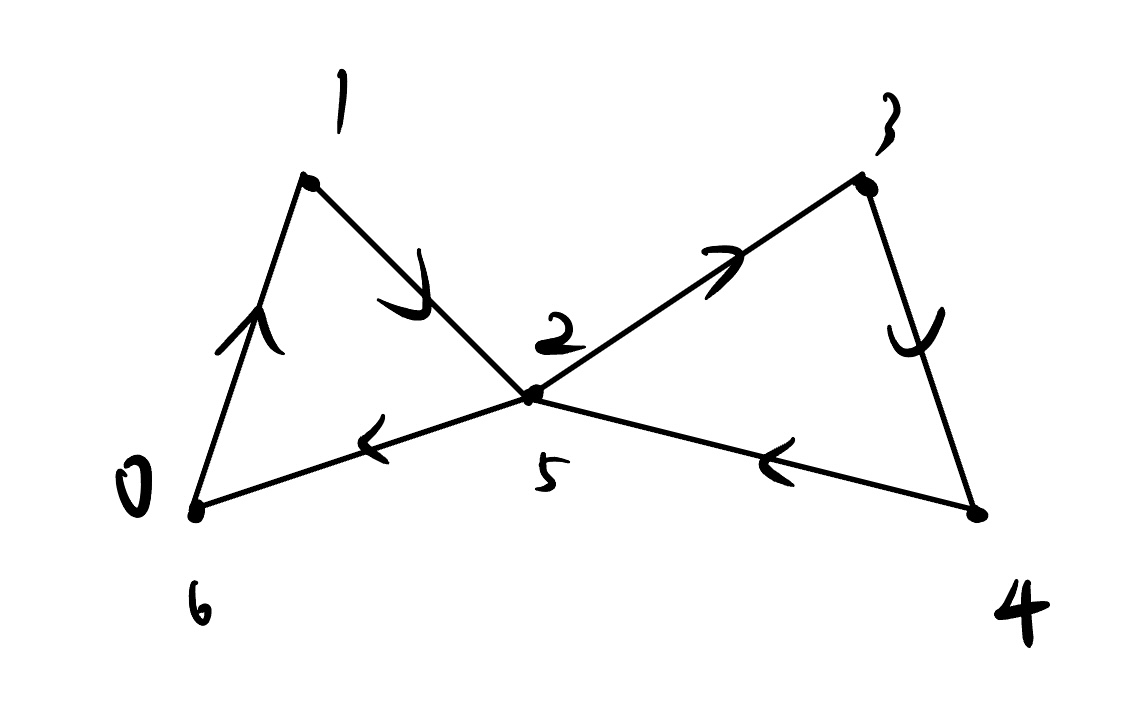
\includegraphics[scale=0.125]{Images/circuit.jpg}
    \caption{A picture of a circuit}
\end{figure}


\begin{definition}
    An \textbf{Eulerian graph} is a graph containing an eulerian circuit.
\end{definition}

\begin{theorem}
    A connected graph $G=(V,E)$ is Eulerian if and only if all its vertices have even degree.
\end{theorem}
\begin{proof}
    (Only If)\\
    Assume $G$ is Eulerian. Note that in an Eulerian trail, for every vertex $v$, each time we enter the vertex, we must leave.(else we've stuck). 
    Hence the vertex must be of even degree.\\
    (If)\\
    Strong induction on the number of edges.\\
    Base case: $t=0$ edges, it is trivial.\\
    Inductive step: Assume for all graphs with $<t$ many edges the if direction is true. 
    Take a connected graph $G=(V,E)$ with $t$ edges. 
    By the procedure defined in the last section, we can prove that $G$ has a cycle subgraph $(\{x_1,\cdots,x_k\},E')$. 
    Consider the connected components of the graph $(V,E \setminus E')$ call them $S_1,\cdots,S_m$.
    \begin{figure}[ht]
        \centering
        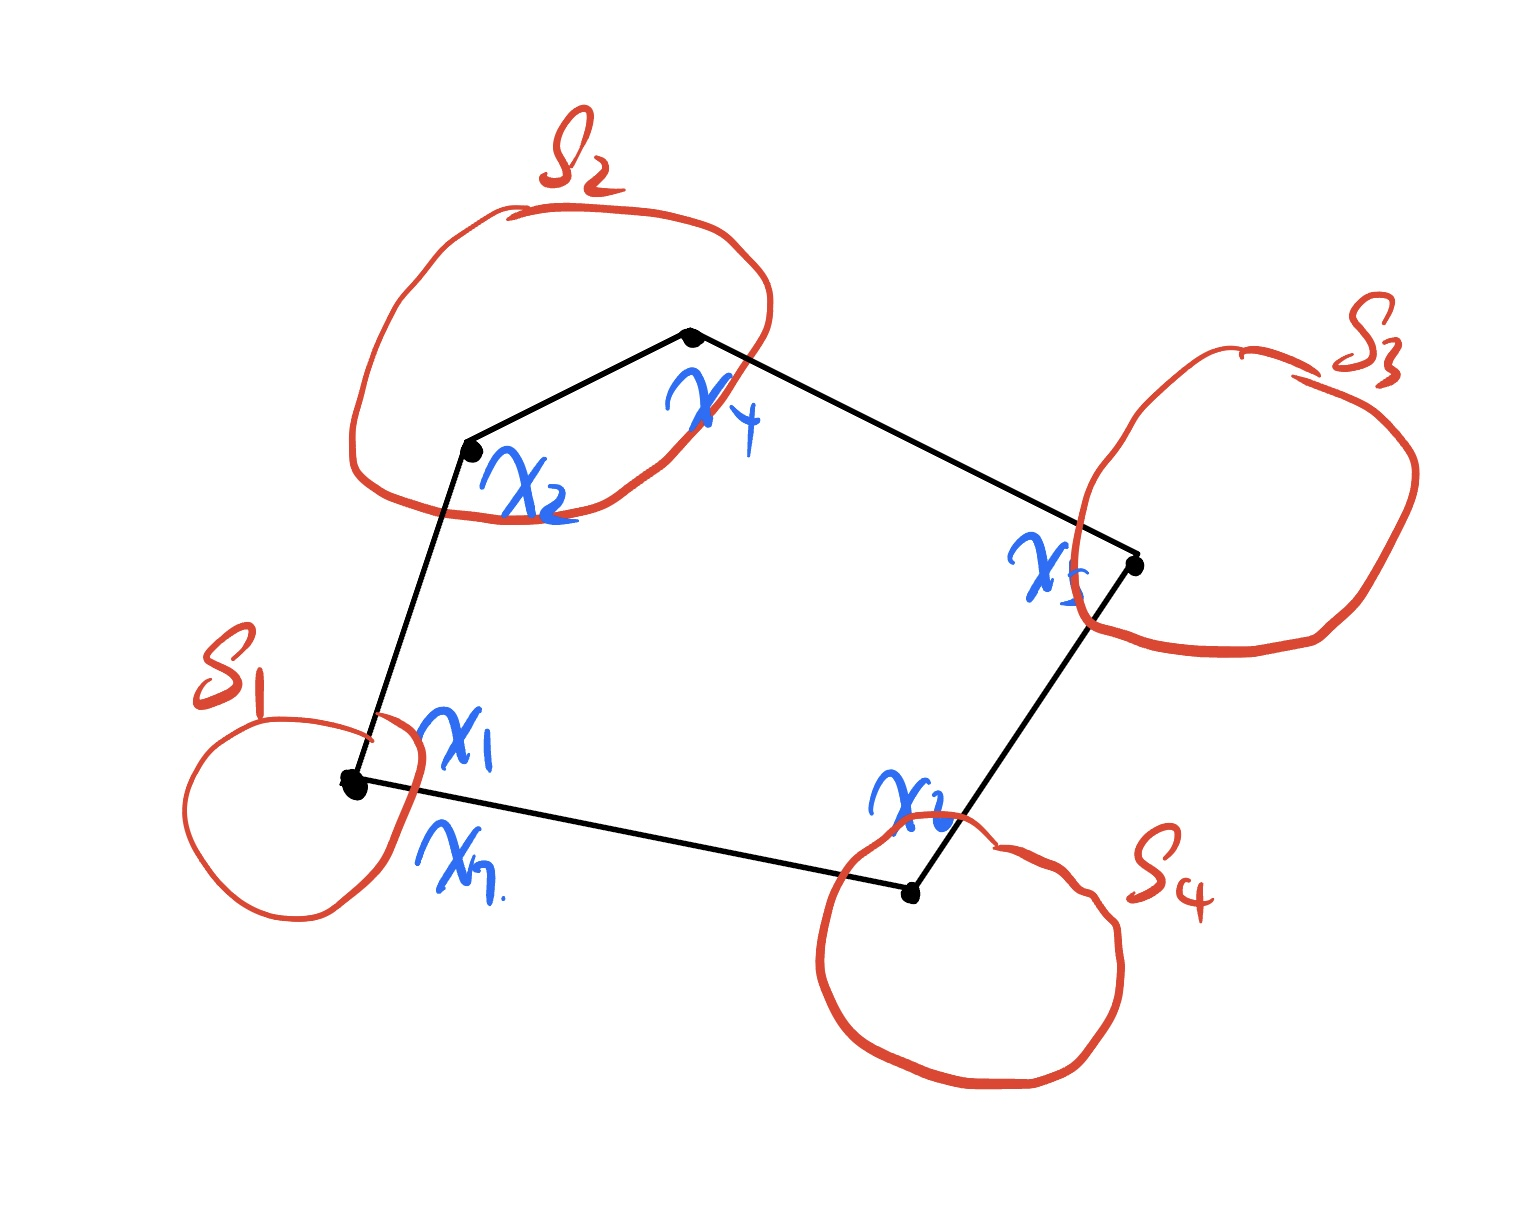
\includegraphics[scale=0.125]{Images/IMG_0298.jpg}
        \caption{A picture discription of our proof}
    \end{figure}
    Start with $x_1$ and the component it is in. Can find an Eulerian circuit back to $x_1$.
    Move from $x_1$ to $x_2$ along the edge $\{x_1,x_2\} \in E'$. 
    If $x_2$ and $x_1$ are in the same connected component, move to $x_3$ and reiterate the argument, else apply induction hypothesis again. 
    We've recursively constructed a sequence $x_1,\cdots,x_1,x_t,\cdots,x_t,\cdots,x_p,\cdots,x_p$ that walks over every edge. 
\end{proof}


\section{Hamiltonian Graphs}

\begin{definition}
    A \textbf{cycle} in a graph $G$ is a sequence of distinct vertices $v_1,\cdots,v_k$ such that for $i \in \{1,\cdots,k-1\}. \{v_i,v_{i+1}\} \in E$ and $\{v_k,v_1\} \in E$.
\end{definition}
\textbf{Note}:
\begin{itemize}
    \item A cycle induces a copy of a subgraph isomorphic to $C_k$ when $k \geq 3$.
    \item We allow for a one point cycle.
\end{itemize}

\noindent \textbf{Remark*}:
\begin{itemize}
    \item Walk: Vertices may repeat. Edges may repeat.(Closed or Open)
    \item Trail: Vertices may repeat. Edges cannot repeat.(Open)
    \item Circuit: Vertices may repeat. Edges cannot repeat.(Closed)
    \item Path: Vertices cannot repeat. edges cannot repeat.(Open)
    \item Cycle: Vertices cannot repeat. Edges may repeat.(Closed)
\end{itemize}

\begin{definition}
    We call a graph with $n$ vertices \textbf{Hamiltonian} if it admits a cycle of length $n$. i.e. it has a spanning subgraph that is isomorphic to $C_n$.
\end{definition}
\begin{figure}[ht]
    \centering
    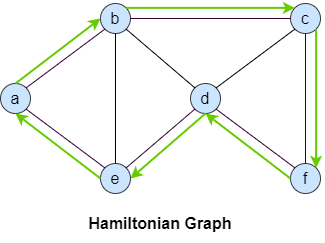
\includegraphics[scale=0.45]{Images/hamiltonian.png}
    \caption{A picture of a Hamiltonian graph}
\end{figure}



\begin{theorem}[Sufficient condition for hamiltonian]
    Let $G=(V,E)$ be a graph with $n$ vertices. Suppose that $\forall v \in V.deg(v) \geq \lceil \frac{n}{2} \rceil$. Then $G$ is Hamiltonian.
\end{theorem}
\begin{proof}
    Since the graph $G$ is finite. We can take a maximal path $v_1,\cdots,v_k$. 
    Note, it must be the case that all the vertices adjacent to $v_1$ or $v_k$ excluding possible each other must be in the sequence $v_2,\cdots,v_{k-1}$. Else we can extand the sequence getting a contradiction.
    There is a $j \in \{2,\cdots,k-1\}$ such that $\{v_1,v_{j-1}\},\{v_j,v_k\} \in E$. 
    If not, (i.e. $\forall j \in \{2,\cdots,k-1\}.\{v_1,v_{j+1}\} \notin E \text{ or } \{v_j,v_k\} \notin E.$) there are $deg(v_1)$ vertices adjacevt to $v_1$. 
    Hence there are $deg(v_1)=\lceil \frac{n}{2} \rceil$ vertices not adjacent to $v_k$. 
    Therefore, there are at least $deg(v_1)+deg(v_k)=\lceil \frac{n}{2} \rceil + \lceil \frac{n}{2}\rceil \geq n$ vertices. 
    Include $v_k$, there are at least $n+1$ vertices. Contradiction.
    \begin{itemize}
        \item It follows that $v_1,\cdots,v_j,v_k,v_{k-1},\cdots,v_{j+1}$ is a cycle.
        \item It follows that every vertex must be on the cycle, else starting from the vertex and moving into the cycle we can create a path of length $>k$.
        \begin{figure}[ht]
            \centering
            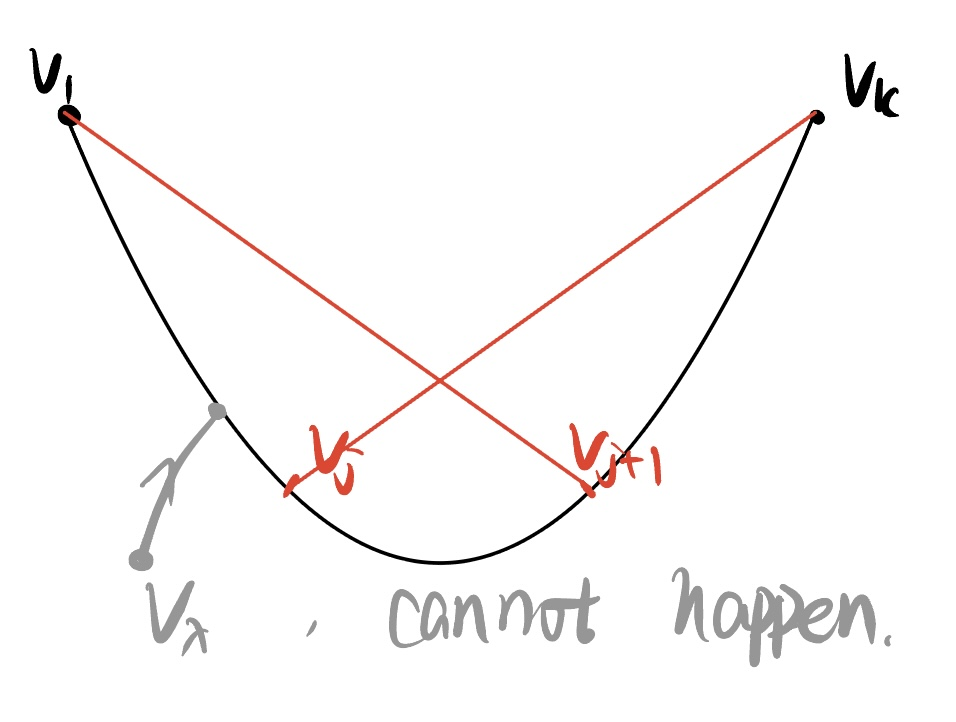
\includegraphics[scale=0.13]{Images/IMG_0299.jpg}
            \caption{A picture discription of the proof}
        \end{figure}
        
    \end{itemize}
\end{proof}


\section{Graph Coloring}

\begin{definition}
    Given a graph $G=(V,E)$, we say $A \subset V$ is \textbf{independent} if and only if no two vertices in $V$ are adjacent.
\end{definition}
\begin{figure}[ht]
    \centering
    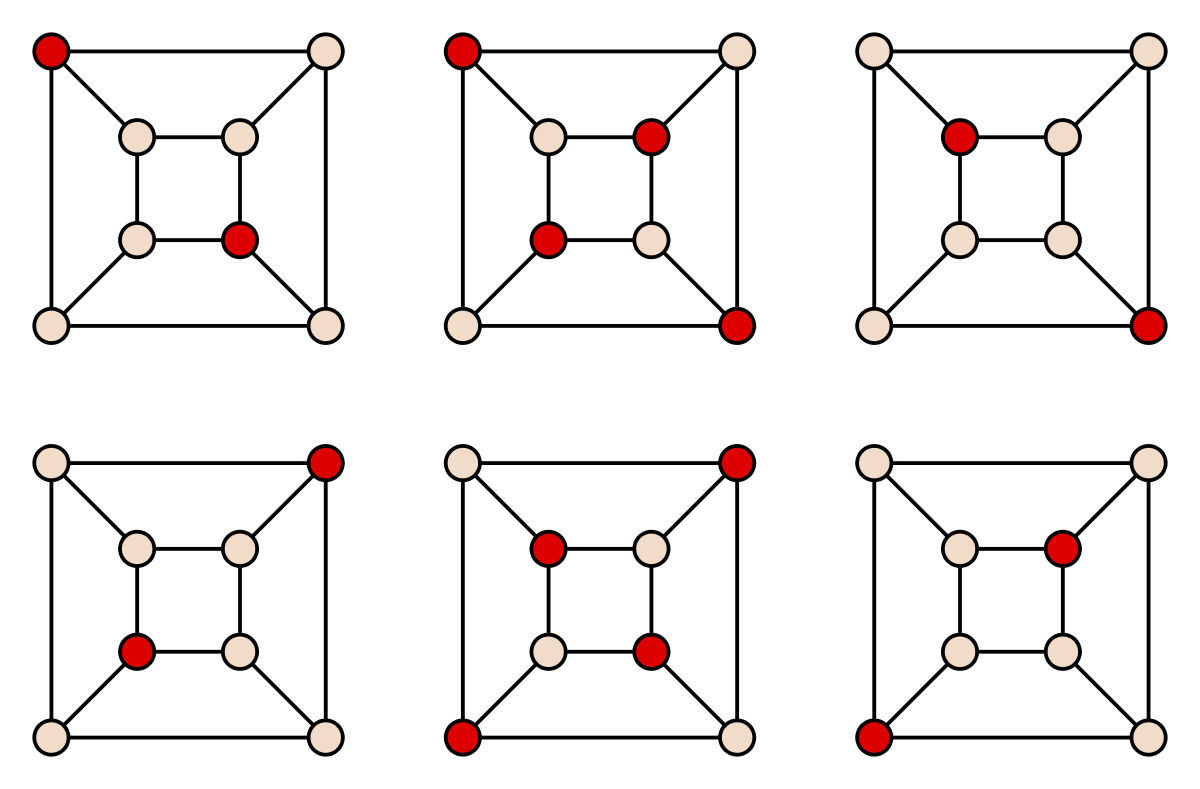
\includegraphics[scale=0.14]{Images/1200px-Cube-maximal-independence.svg.png}
    \caption{A picture independent parts}
\end{figure}
\textbf{Remark}:
\begin{itemize}
    \item If we think the graph that represent the relations of people, then the independent set represent a set of people who don't know each other.
    \item Can show that the only independent sets in $K_n$ are singletons.
\end{itemize}

\begin{definition}
    We say a graph $G=(V,E)$ is \textbf{bipartite} if and only if we can partition $V$ into two disjoint independent sets.
\end{definition}
\textbf{Question}:
\begin{itemize}
    \item Show that a graph is bipartite if and only if it does not contain a cycle of odd length.
\end{itemize}
\begin{figure}[ht]
    \centering
    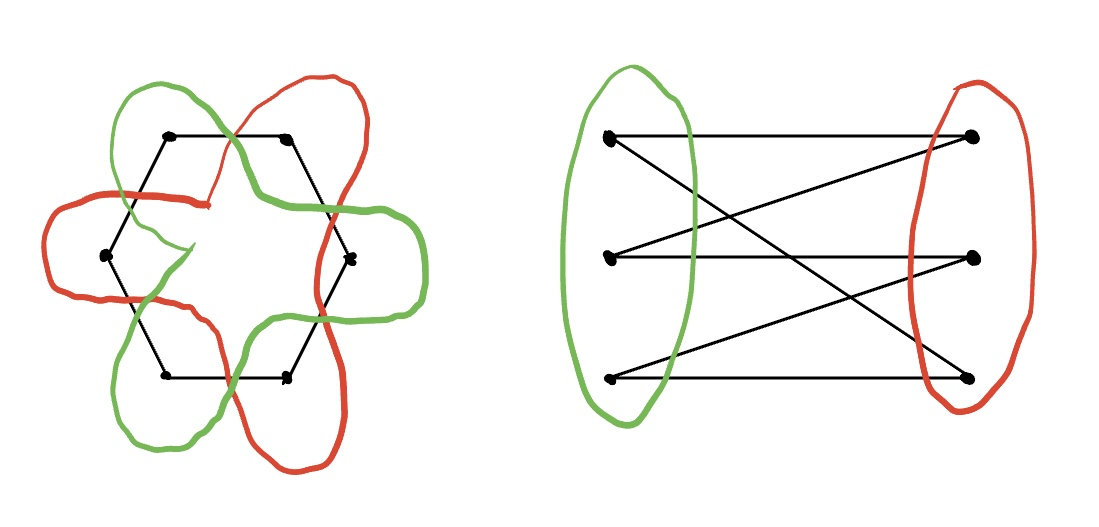
\includegraphics[scale=0.2]{Images/IMG_0300.jpg}
    \caption{A picture bipartite graphs}
\end{figure}

\begin{definition}
    A \textbf{complete bipartite graph} $K_{n,m}=([n]\cup[m],E)$ is a special bipartite graph where every vertex of the $[n]$ is connected to every vertex of $[m]$ and vice versa.
\end{definition}
\begin{figure}[ht]
    \centering
    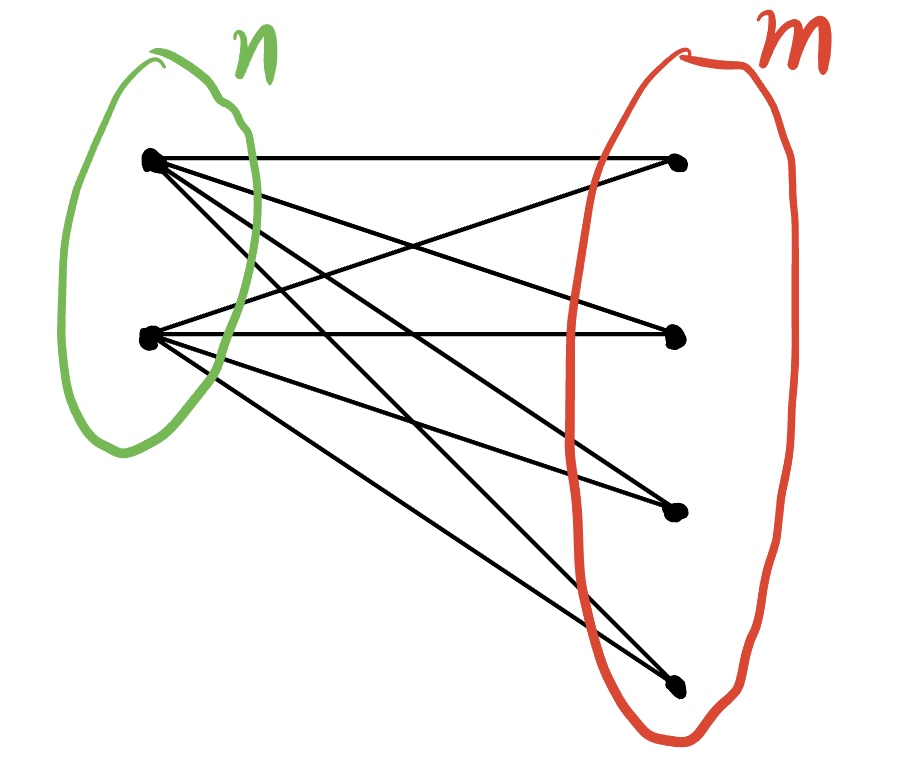
\includegraphics[scale=0.14]{Images/IMG_0301.jpg}
    \caption{A picture of $K_{2,4}$}
\end{figure}


\begin{definition}
    Let $G=(V,E)$ be a graph. A \textbf{(proper) colouring} of $G$ is a function $$\phi:V \longrightarrow [k]$$
    such that for all $i \in [k]$, $\phi^{-1}(i)$ is independent. 
    Equivalently, if $\{a,b\}\in E$,$\phi(a) \neq \phi(b)$, we call $\phi$ a \textbf{k-colouring}.
\end{definition}
\begin{figure}[ht]
    \centering
    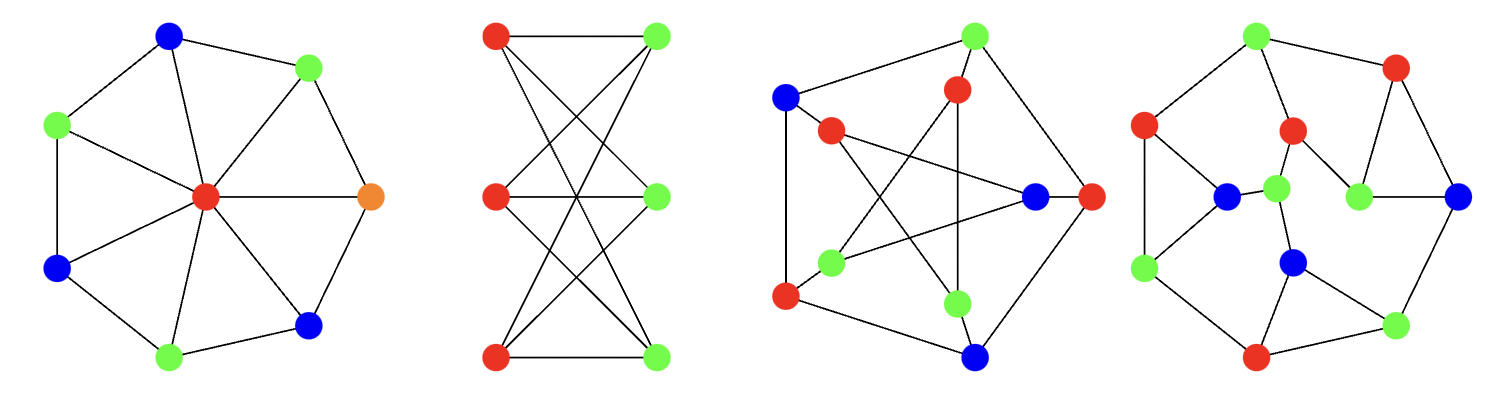
\includegraphics[scale=0.35]{Images/colouring.png}
    \caption{A picture of colouring}
\end{figure}


\begin{definition}
    \textbf{The chromatic number} of a graph $G$, is the smallest $k$ such that there is a proper k-colouring of $G$. 
    We denote this number \underline{$\chi(G)$}
\end{definition}

\begin{definition}
    We say a graph $G$ is \textbf{planar} if there exists a depiction of it on a plane without any edge crossing.(i.e. you can draw it on a piece of paper with no edge crossing)
\end{definition}
\textbf{Remark}:
\begin{itemize}
    \item The above should feel unsatisfactory due to lack of mathematical rigidity. This issue is solved thanks to Kuratowski.
    \item The key inthe above definition is the existence.
\end{itemize}
\begin{figure}[ht]
    \centering
    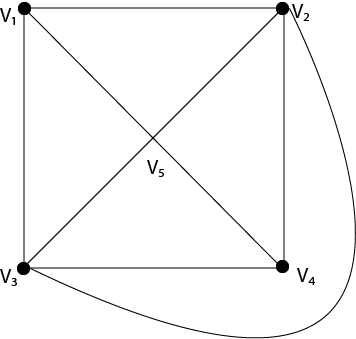
\includegraphics[scale=0.3]{Images/planar-and-non-planar-graphs2.png}
    \caption{$K_4$ is planar}
\end{figure}
\textbf{Real world applications}:
\begin{itemize}
    \item In computer science, there is a notation of \underline{thickness} that correlates planarity to how difficult a network is to embed.
    $$\text{\underline{How many planar pieces I can cover a graph with.}}$$
    For optimization problems, if you have a complicated network or a system that you need to embed on a plane or some circuit board, you should know how many boards you need,
    \item Questions of circuitry lines or wires are not allowed to cross are questions on planarity.(when the circuits must be embedded or built into a relatively 2D configuration)
\end{itemize}

\begin{definition}
    A \textbf{face} is a region bounded by edges in a planar depiction
\end{definition}
\begin{figure}[ht]
    \centering
    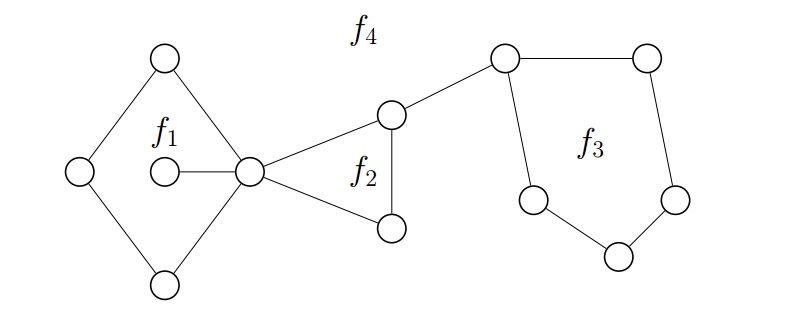
\includegraphics[scale=0.4]{Images/lrgtF.jpg}
    \caption{A planar embedding with 4 faces}
\end{figure}
\textbf{Remark}:
\begin{itemize}
    \item There is a basis of non-planar graphs.
\end{itemize}

\begin{definition}[Euler's Formula]
    Given a connected planar graph $G$ with $n$ vertices, $m$ edges, and $f$ faces. Then $$n-m+f=2$$
\end{definition}
\begin{proof}
    Do induction on $m$.\\
    Base case: $m=0$, the graph is a singleton. $1-0+1=2$ as desired.\\
    Inductive step: Suppose the assertion is true for graphs with $m$ edges. 
    Suppose $G$ is a graph with $m+1$ edges.
    \begin{itemize}
        \item If we can remove an edge in such a manner that keeps the graph connected, said edge must divide some face into two,so we get a new graph with $n$ vertices, $m$ edges and $f'=f-1$ faces. 
        By induction hypothesis, $n-m+f-1=2$. Hence we have $n-(m+1)+f=2$.
        \item Else, the graph is a tree and we're done as trees have 1 face.(the outer face, and any other face generates a cycle).
    \end{itemize}
\end{proof}

\begin{corollary}
    Let $G$ be a planar graph with $n \geq 3$ vertices and $m$ edges. We have the bound $$m \leq 3n-6$$
\end{corollary}
\begin{proof}
    Suppose the graph is connected and not a tree. (As it is trivial in the case for tree $m=n-1<3n-6$ for $n \geq3$)
    Let $S$ be the collection of pairs $(e,F)$ where $e$ is an edge and $F$ is a face.
    \begin{figure}[ht]
        \centering
        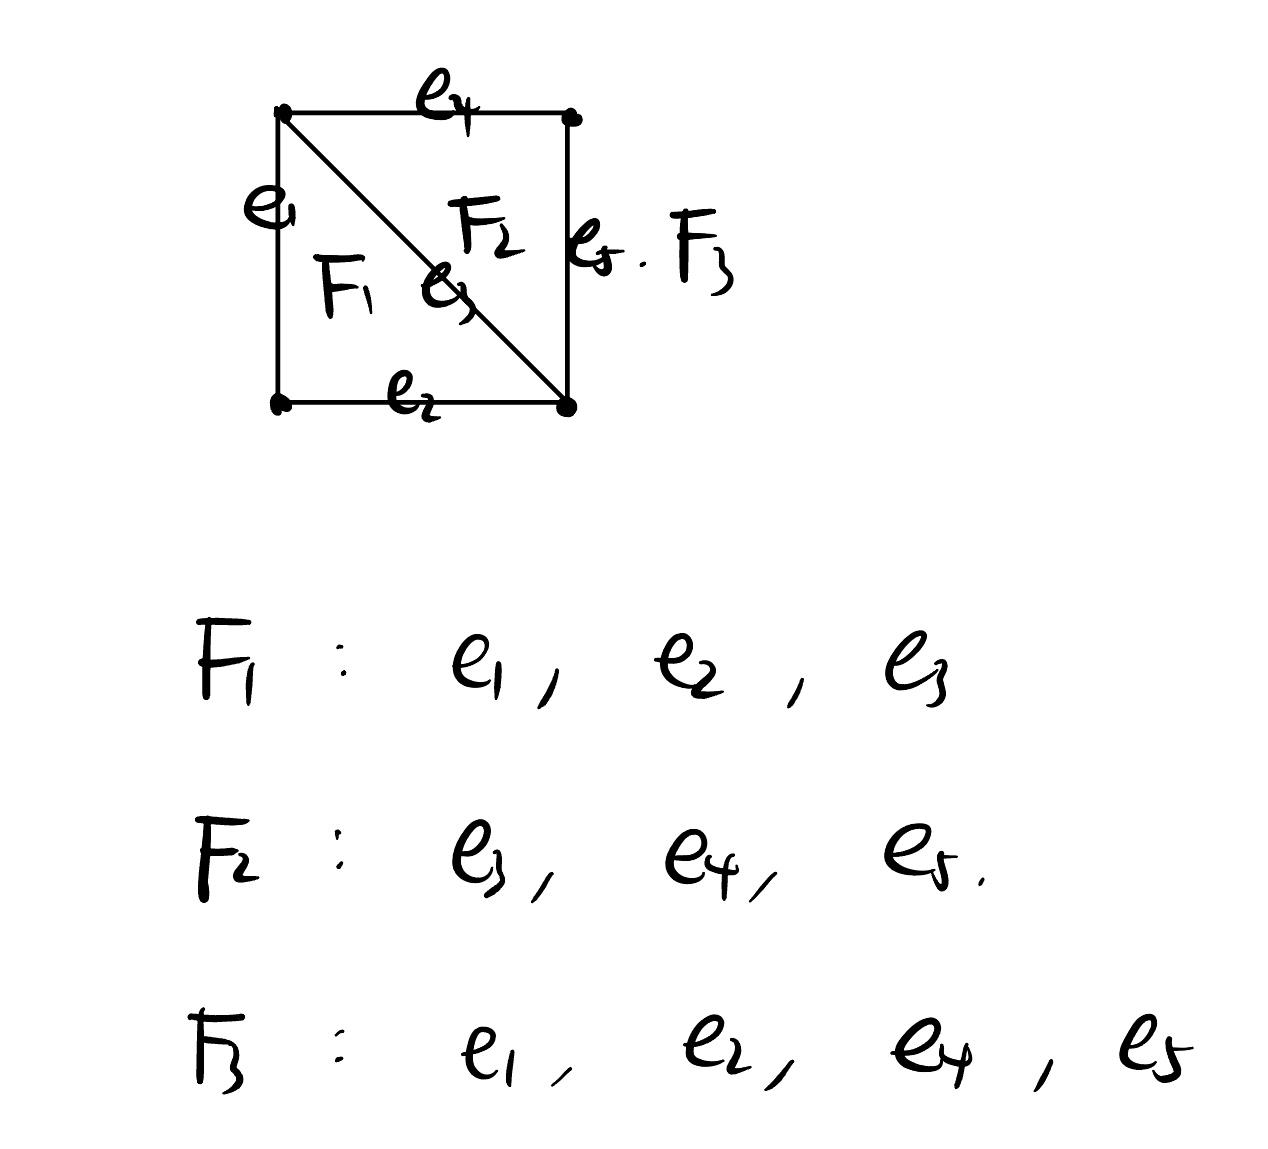
\includegraphics[scale=0.15]{Images/IMG_0303.jpg}
        \caption{A picture discription}
    \end{figure}
    \begin{itemize}
        \item For a fixed $e$, $|\{F:(e,F)\in S\}| \leq2$ as an edge borders at most 2 faces.
        \item For a ficed $F$, $|\{e: (e,F)\in S\}| \geq 3$
    \end{itemize}
    It follows that $3f \leq|S|\leq 2m$. By Euler's formula $$m=n+f-2 \leq n +\frac{2}{3}m-2$$
    This implies $m \leq 3n-6$. Complete proof in case of disconnectivity.(Breaking into connected components, and using the above)
\end{proof}
\textbf{Remark}:
\begin{itemize}
    \item Can use this to decide whether a graph is planar. For $K_5$, $m=10 >3\times5-6=9$, so $K_5$ is not planar.
\end{itemize}

\begin{definition}
    Let $G=(V,E)$ be a graph and take $e \in E$ and edge(set of 2 vertices). 
    A \textbf{contraction along e} is a graph $G'=((V\setminus e)\cup \{e\}, E')$
    where we say for all $u,v \in V \setminus e$, 
    $$\{u,v\}\in E \Longleftrightarrow \{u,v\}\in E'$$ and
    $$\{u,e\}\in E' \Longleftrightarrow \exists x \in e. \{u,x\}\in E$$
\end{definition}
\begin{figure}[ht]
    \centering
    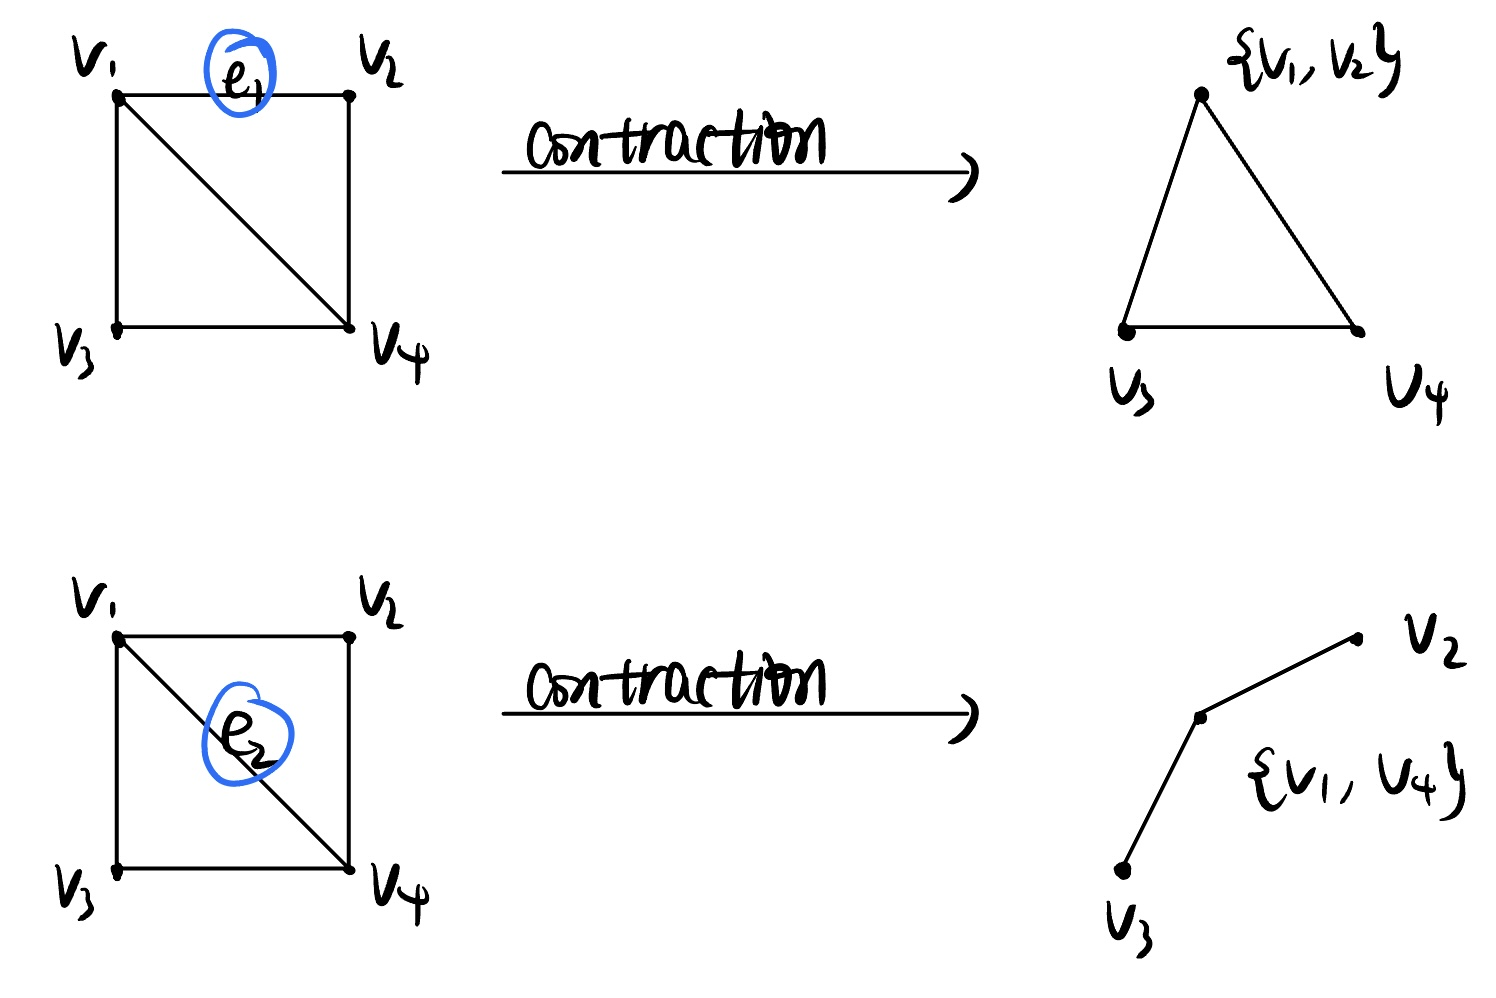
\includegraphics[scale=0.15]{Images/IMG_0304.jpg}
    \caption{A picture of contraction}
\end{figure}
\textbf{Remark}:
\begin{itemize}
    \item The essence is taking two vertices on that edge, and suck them together, Some people refer this as \underline{smoothing}.
\end{itemize}

\begin{definition}
    A \textbf{graph minor} of a graph $G$ is a graph $H$ gotten via a process of taking subgraphs and contractions.
\end{definition}

\begin{theorem}[Kuratowski]
    A graph is planar if and onlt if it does not contain a copy of $K_5$ or $K_{3,3}$ as a minor.
\end{theorem}
\begin{figure}[ht]
    \centering
    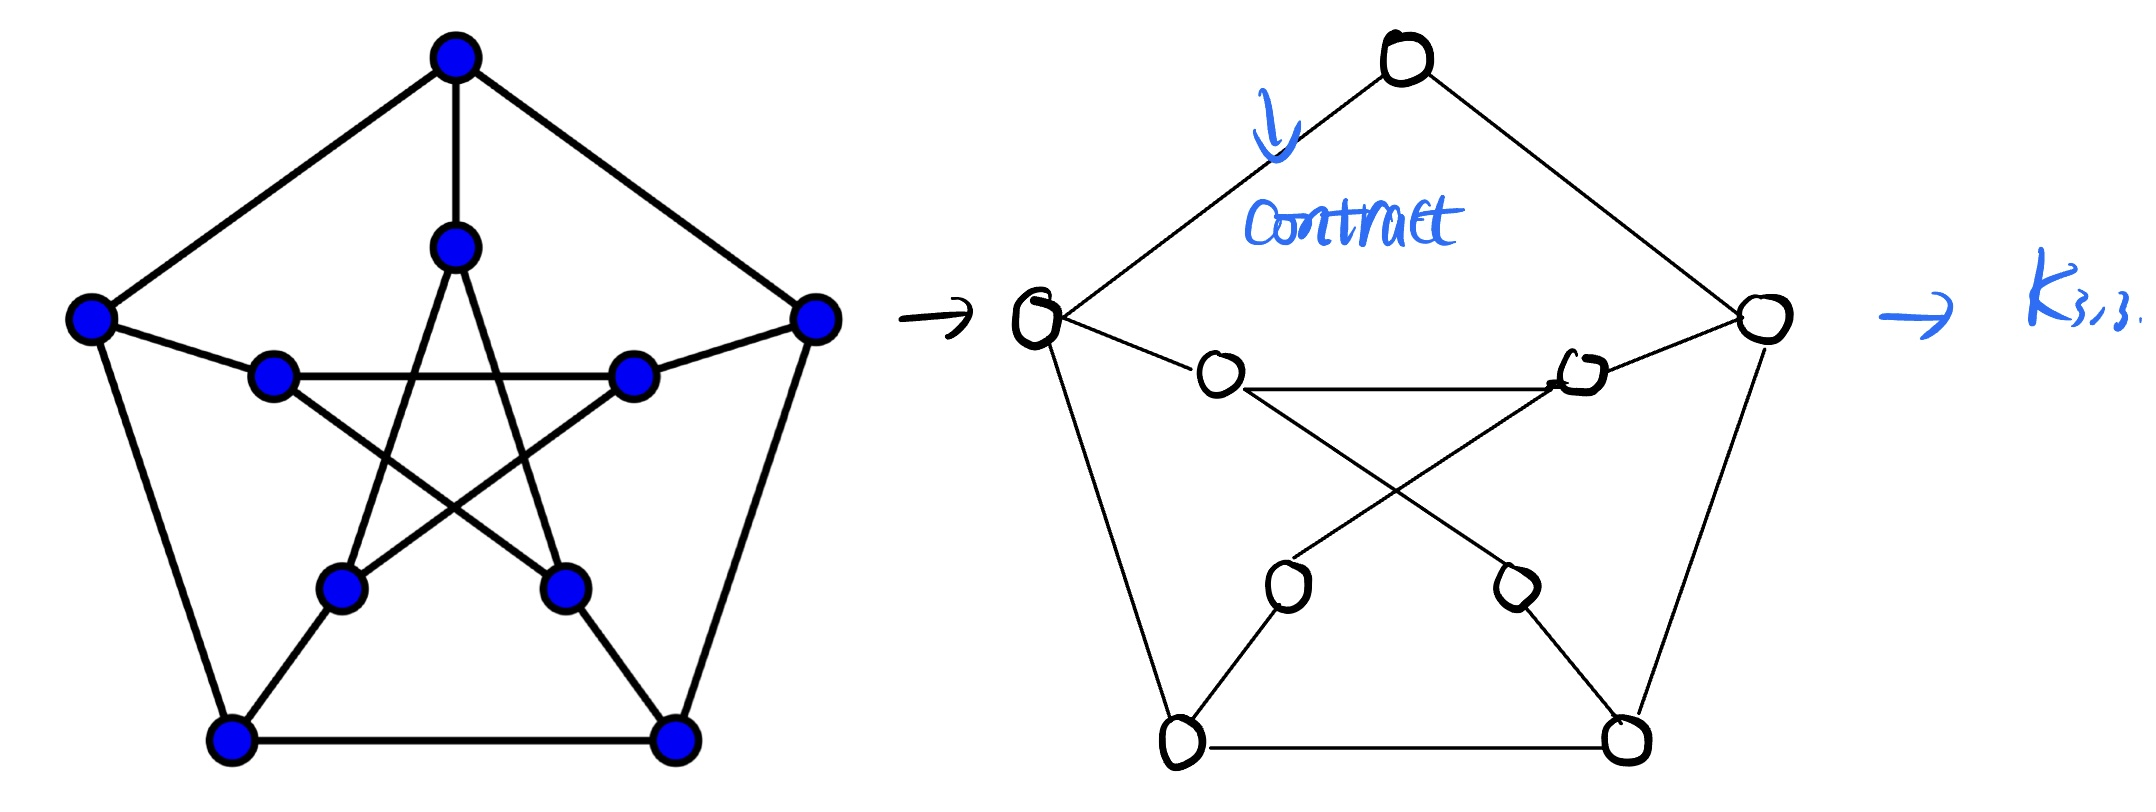
\includegraphics[scale=0.14]{Images/IMG_0305.jpg}
    \caption{Petersen graph is not planar}
\end{figure}

\begin{theorem}
    Let $G$ be a graph. If $G$ is planar, then $\chi(G) \leq4$.
\end{theorem}
\textbf{Remark}:
\begin{itemize}
    \item This was proved via brute force computational methods.
    \item Still open if solvable without extreme case work.
\end{itemize}


\section{Posets}

\begin{definition}
    A \textbf{partially ordered set(poset)} is a pair $\mathbb{P}=(X,P)$ where $X$ is a set and $P \subset X^2$ is a relation that is:
    \begin{itemize}
        \item \underline{Reflexive}: $\forall a \in X. (a,a)\in P$
        \item \underline{Anti-symmetric}: if $a \neq b$ with $(a,b)\in P$, then $(a,b)\notin P$
        \item \underline{Transitive}: if $(a,b)\in P$ and $(b,c)\in P$, then $(a,c) \in P$
    \end{itemize}
\end{definition}
\textbf{Remark}:
\begin{itemize}
    \item Instead writing $(a,b)\in P$, we adopt the notation $a \leq_{\mathbb{P}}$.
    \item Having the subscript is useful. Don't confuse poset orders with more classic orders, though it is acceptable to write $a \leq b$.
\end{itemize}

\begin{definition}
    Given a poset $\mathbb{P}=(X,P)$ and $\mathbb{Q}=(Y,Q)$, an \textbf{embedding} from $\mathbb{P}$ to $\mathbb{Q}$ is an injective map:$f:X \longrightarrow Y$ with the property that $$a \leq_{\mathbb{P}} b \Longleftrightarrow f(a) \leq_{\mathbb{Q}} f(b)$$
    \begin{itemize}
        \item If the embedding is surjective, we call it \textbf{isomorphism}.
        \item If $\mathbb{P}=\mathbb{Q}$, we call it \textbf{automorphism(self isomorphism)}.
    \end{itemize}
\end{definition}

\begin{definition}
    Given a poset $\mathbb{P}=(X,P)$, we call the poset $\mathbb{P}^d=(X,P^d)$ given by $$a \leq_{\mathbb{P}^d} b \Longleftrightarrow b \leq_{\mathbb{P}} b$$
    the \textbf{dual} of $\mathbb{P}$. we say a poset is \textbf{self-dual} if it is isomorphic to its dual.
\end{definition}

\begin{definition}
    Given a poset $\mathbb{P}=(X,P)$ and a point $a \in X$, we say $a$ is \textbf{covered} by a point $b \in X$ if $a <_{\mathbb{P}} b$ and there is no $c$ such that $a <_{\mathbb{P}} c <_{\mathbb{P}} b$.
\end{definition}
\textbf{Remark}:
\begin{itemize}
    \item $b$ is directly above $a$, nothing between, but not necessarily unique.
\end{itemize}

\begin{definition}
    Given a poset $\mathbb{P}=(X,P)$, we call the graph $G=(X,E)$ given by $$\{x,y\}\in E \Longleftrightarrow x \text{ covers }y \text{ or }y \text{ covers }x$$
    the \textbf{cover graph} associated to $\mathbb{P}$.
\end{definition}
\textbf{Remark}:
\begin{itemize}
    \item We can draw the graph in an oriented fashion in which lower vertices correspond to $\leq_{\mathbb{P}}$-smaller elements. We call this depiction a \textbf{Hasse diagram}.
\end{itemize}


\begin{definition}
    Given a poset $\mathbb{P}=(X,P)$, we say two points $a,b \in X$ are \textbf{comparable} if either $$a <_{\mathbb{P}} b \text{ or } b<_{\mathbb{P}} a$$
    If two points are not comparable, we call them \textbf{incomparable}.
\end{definition}


\begin{definition}
    Given a poset $\mathbb{P}$, we say $\mathbb{P}$ is \textbf{linearly ordered} if no two distinct points are incomparable.
\end{definition}
\textbf{Questions}:
\begin{enumerate}
    \item Show that there is only one linear order of size $n$ up to isomorphism.
    \item Show that any linear order is self-dual.
\end{enumerate}


\begin{definition}
    Given a poset $\mathbb{P}$, we call $C \subset X$ a \textbf{chain} if every pari of distinct elements are comparable. 
    We call $A \subset X$ an \textbf{antichain} if every pair of elements in $A$ are incomparable.
\end{definition}


\begin{definition}
    Given a poset $\mathbb{P}$, we define the parameters \textbf{width} and \textbf{height} to denote the size of the largest antichain and chain respectively.
\end{definition}


\begin{theorem}[Spencer]
    Consider the poset $\mathbb{P}=(\mathcal{P}([n]), \subseteq)$, then $$width(\mathbb{P})={n \choose \lfloor \frac{n}{2} \rfloor}$$
\end{theorem}
\begin{proof}
    One can easilly verify $A=\{S \subset \mathcal{P}([n]):|S|=\lfloor \frac{n}{2} \rfloor\}$ is an antichain. (two sets of the same size are comparable iff they are equal.). 
    So $$width(\mathbb{P}) \geq {n \choose \lfloor \frac{n}{2} \rfloor}$$
    Take $A=\{S_1,\cdots,S_w\}$ be a maximal antichain of $\mathbb{P}$, each $S_i \subset [n]$. 
    Consider for each $i \in\{1,\cdots,w\}$, $C_i$ is the set of maximal chains such that $S_i \in C_i$.
    \begin{figure}[ht]
        \centering
        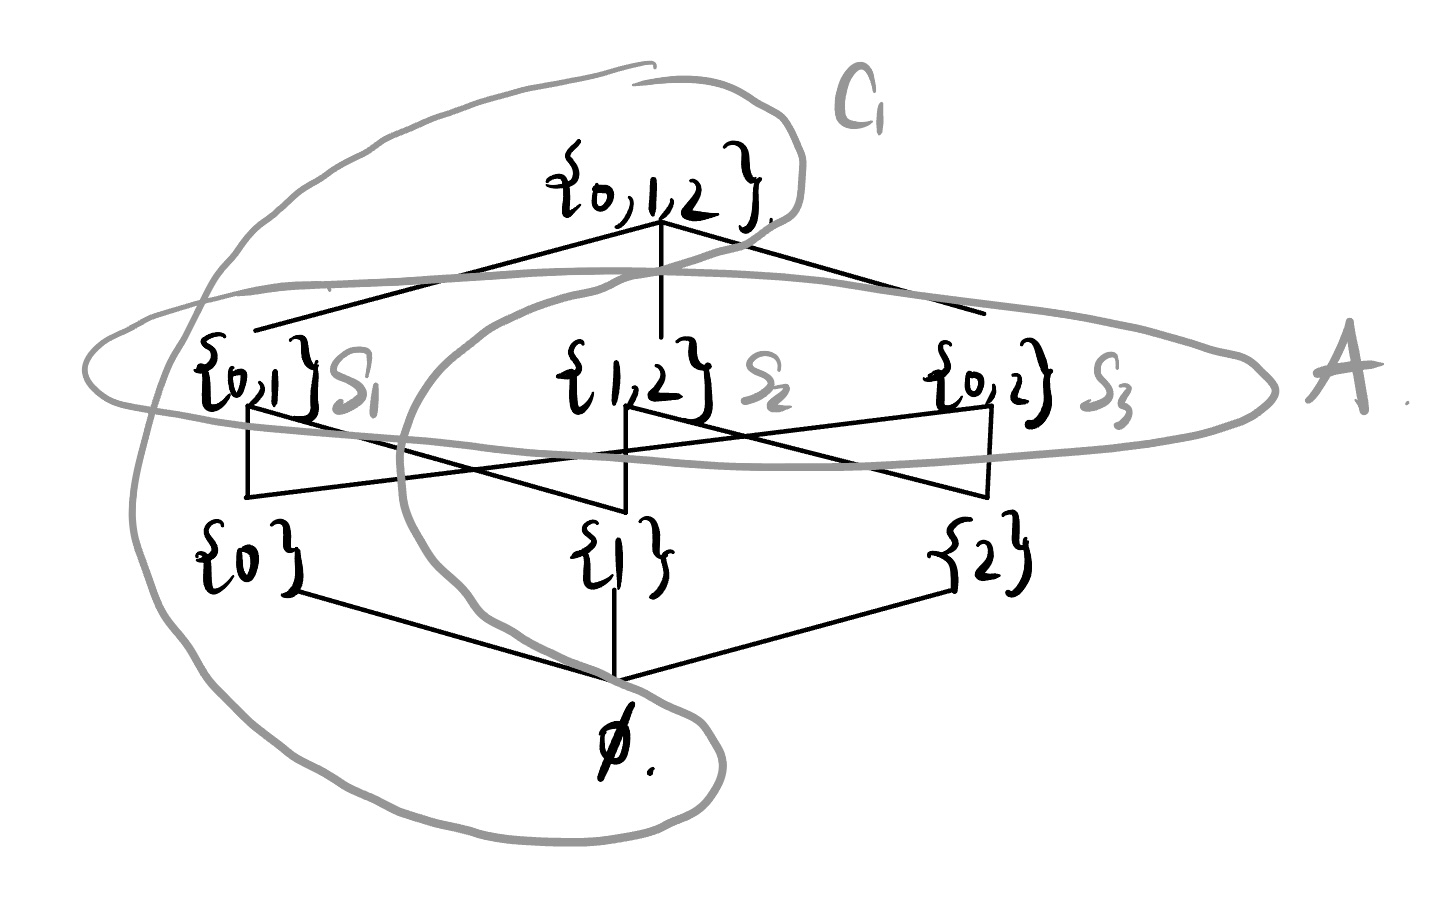
\includegraphics[scale=0.15]{Images/IMG_0306.jpg}
        \caption{A picture discription of the proof}
    \end{figure}
    For any $i$ we have $$|C_i|=|S_i|!(n-|S_i|)!$$ As a maximal chain must be an $\subseteq$-increasing sequence that differs by at most one element per successive cover. 
    There are $(k-|S_i|)!$ many ways to add points successively to $S_i$ and $|S_i|!$ many ways to remove points from $S_i$ successively. 
    Similarly, there are exactly $n!$ many maximal chains.
    \begin{figure}[ht]
        \centering
        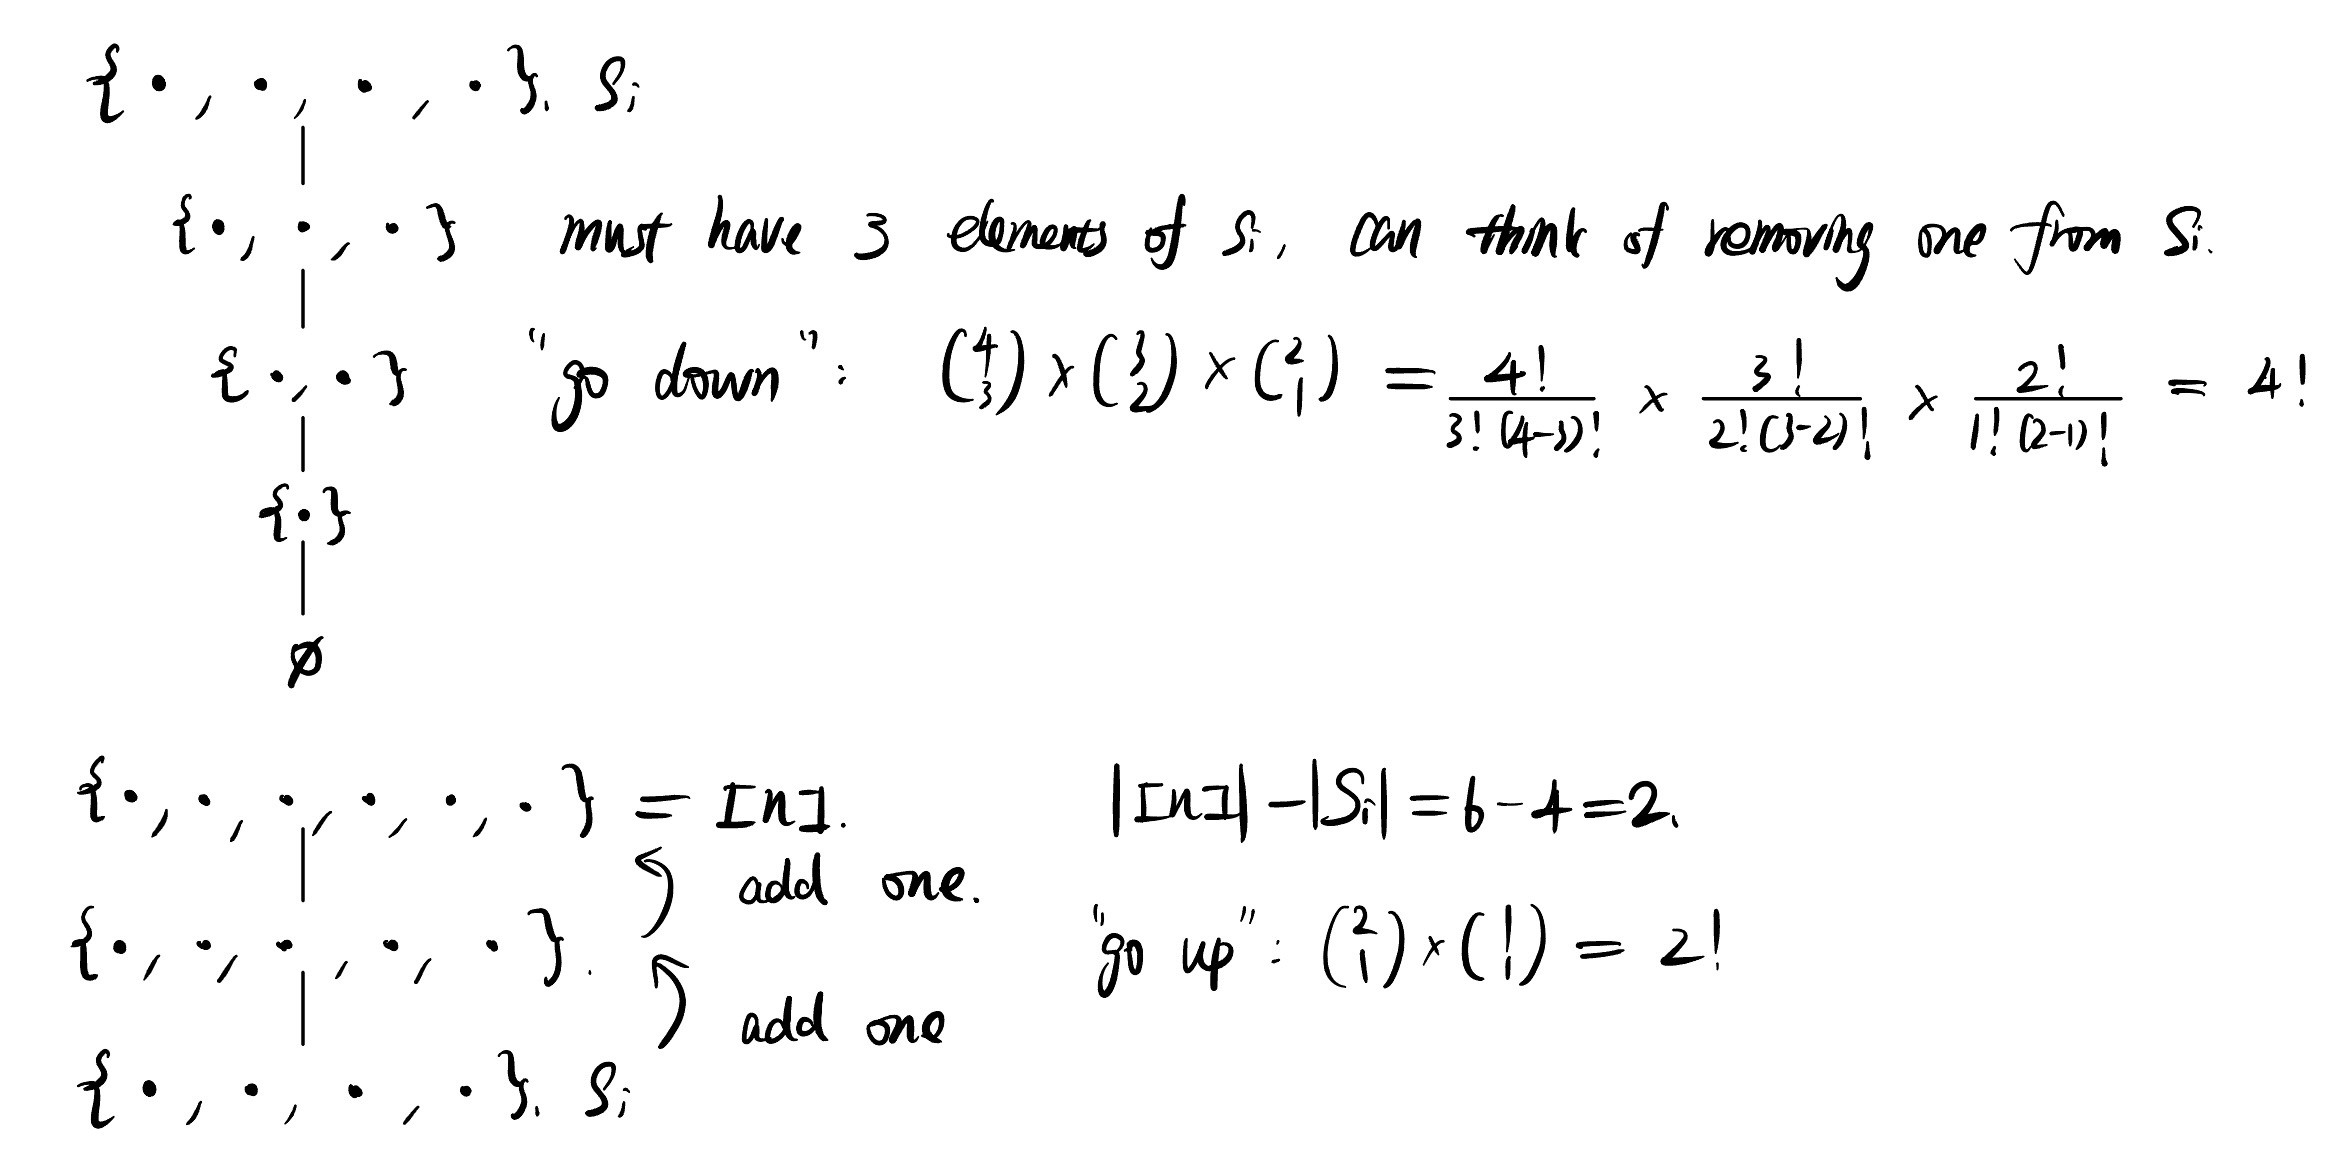
\includegraphics[scale=0.15]{Images/IMG_0307.jpg}
        \caption{A picture discription of the proof}
    \end{figure}
    For any $i \neq j$, $C_i \cap C_j=\{\emptyset,[n]\}$, else there is a chain $C$ with $S_i,S_j \in C$ and hence $S_i$ and $S_j$ are comparable, contradiction. 
    It follows that $$\sum_{i=1}^w|C_i| \leq n!$$ further we have $$\sum_{i=1}^w \frac{|S_i|!(n-|S_i|)!}{n!} \leq 1$$
    hence $$\sum_{i=1}^w \frac{1}{{n \choose |S_i|}} \leq 1$$
    Using that $${n \choose |S_i|} \leq {n \choose \lfloor \frac{n}{2} \rfloor}$$
    we can get the result.
\end{proof}

\begin{theorem}[Mirsky(Dual Dilworth)]
    Let $\mathbb{P}$ be a poset with $height(\mathbb{P})=h$. 
    There is a partition of $X$ into $w$ antichains $A_1,\cdots,A_h$. 
    Moreover, there is optimal in that you cannot cover $\mathbb{P}$ with $<h$ many antichains.
\end{theorem}
\begin{proof}\
    \begin{enumerate}
        \item For each $a \in X$, consider the set $D_a=\{b \in X: b \leq_{\mathbb{P}} a\}$. Let $\mathbb{D}_a=(D_a,P)$.\\
        For each $i \in \{1,\cdots,h\}$, let $A_i=\{a \in X: height(\mathbb{D}_a)=i\}$
        \begin{figure}[ht]
            \centering
            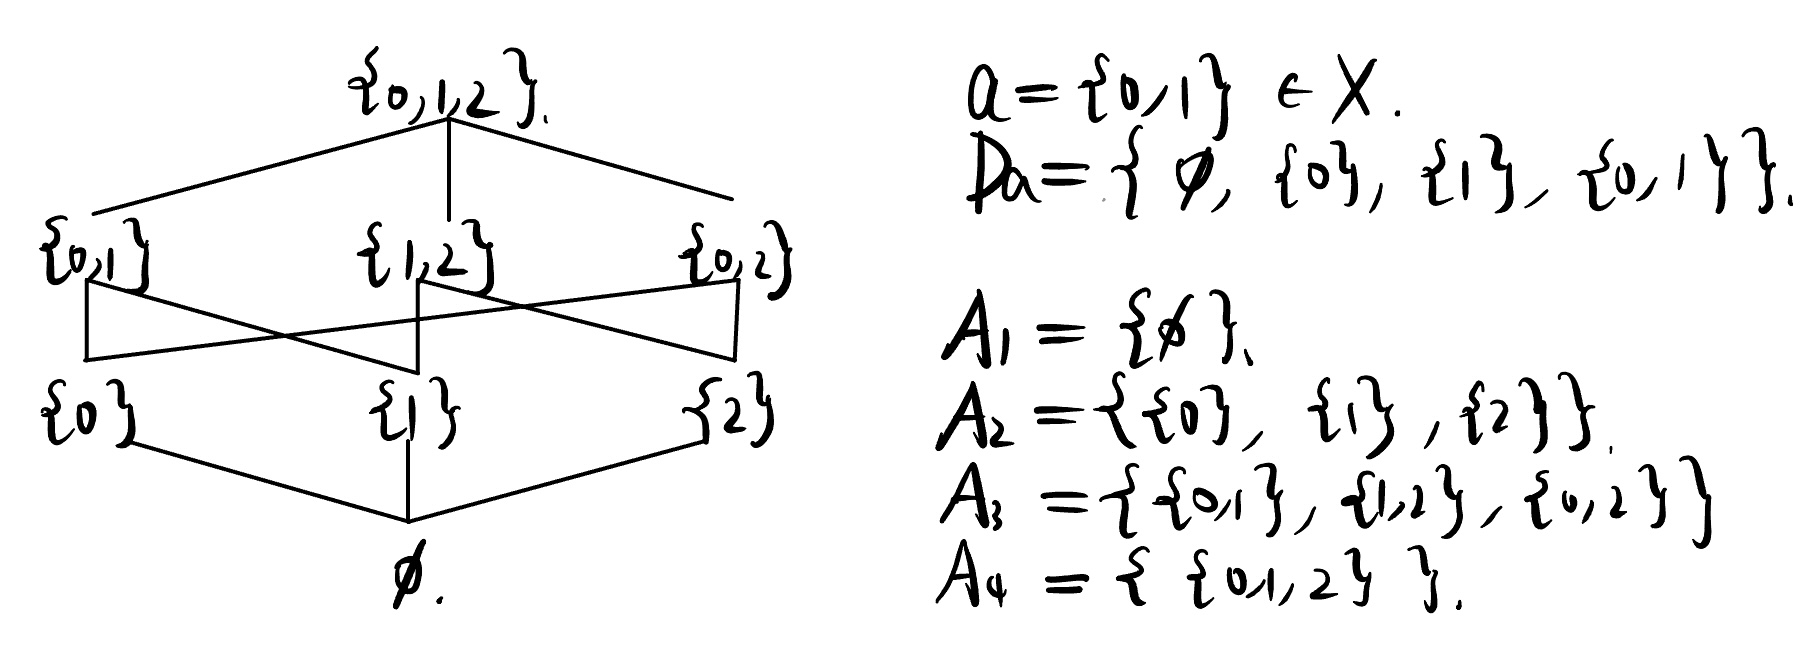
\includegraphics[scale=0.15]{Images/IMG_0310.jpg}
            \caption{A picture discription of the proof}
        \end{figure}
        This forms a proper partition of $X$, as if $|D_a| >h$ for some $a \in X$ would contradict the definition of height. 
        The sets $A_i$ are also antichains. If $height(\mathbb{D}_a)=height(\mathbb{D}_b)$ and $a \in D_b$, then $b \notin D_a$ and $D_a \cup \{b\} \subset D_b$. 
        But then $$height(\mathbb{D}_b) \geq height(\mathbb{D}_a)+1 >height(\mathbb{D}_b)$$
        This is a contradiction.
        \item To see this is optimal, is also by way of contradiction. 
        Suppose we partitioned $X$ into $k$ antichains: $A_1,\cdots,A_k$ for $k < h$. 
        Take a chain $C$ of size $h$ and consider the map $f:C \longrightarrow \{1,\cdots,k\}$ given by $$f(a)=i \Longleftrightarrow a \in A_i$$
        By the Pigeon Hole Principle, there is some $A_i$ that contains two distinct members of $C$, hence the are incomparable. 
        This contradicts to that $C$ is a chain. 
    \end{enumerate}
\end{proof}

\begin{theorem}[Dilworth]
    Let $\mathbb{P}$ be a poset with $width(\mathbb{P})=w$. 
    There is a partition of $X$ into $w$ chains $C_1,\cdots,C_w$. 
    Moreover, there is optimal in that you cannot cover $\mathbb{P}$ with $<w$ many chains.
\end{theorem}
\begin{proof}
    (proceed bt strong induction on $|X|$)\\
    Base case: $|X|=1$. The poset is the one point linear order. So $X$ is a chain itself and we're done.\\
    Inductive step: Take a poset $\mathbb{P}=(X,P)$ with $width(\mathbb{P})=w$ and $hright(\mathbb{P})=h$. 
    Assume the theorem is true for all posets with cardinality $k < |X|$. 
    Let $C=\{x_1,\cdots,x_n\}$ be a maximal chain in $\mathbb{P}$. Consider the subposet $\mathbb{Q}=(X \setminus C, P \cap (X \setminus C)^2)$. 
    Note that $width(\mathbb{Q}) \leq width(\mathbb{P})$. 
    \begin{enumerate}
        \item Case1: $width(\mathbb{Q}) < width(\mathbb{P})$.\\ 
        We claim that $$width(\mathbb{Q})=w-1$$
        By assumption, we have $width(\mathbb{Q})=w' \leq w-1$. Since $height(\mathbb{P})=h$,
        by Mirsky's theorem, we have minimal number of antichains: $A_1,\cdots,A_{h'}$. So $w = max\{|A_1|,\cdots,|A_n|\}$. 
        Since $height(\mathbb{q})=h' \leq h$, by Mirsky's theorem, we have minimal number of antichains:$B_1,\cdots,B_{h'}$. So $w'=max\{|B_1|,\cdots,|B_{h'}\}$. \
        We removed a chain $C$ from $\mathbb{P}$. Can use Pigeon Hole Principle to show that: for each $A_i$, we removed one element. 
        The new $A_i'$s are also antichains which forms a partition for $\mathbb{Q}$. 
        By definitionof width, $$w' \geq max\{|A_1|-1,\cdots,|A_n|-1\}=w-1$$
        Hence $w'=w-1$.\\
        Apply the induction hypothesis to $\mathbb{Q}$, can cover it with $C_1,\cdots,C_{w-1}$ chains. Then $C_1,\cdots,C_{w-1},C$ forms a cover of $\mathbb{P}$ with $w$many chains.
        \item Case2: $width(\mathbb{Q})=width(\mathbb{P})$.\\
        \begin{figure}[ht]
            \centering
            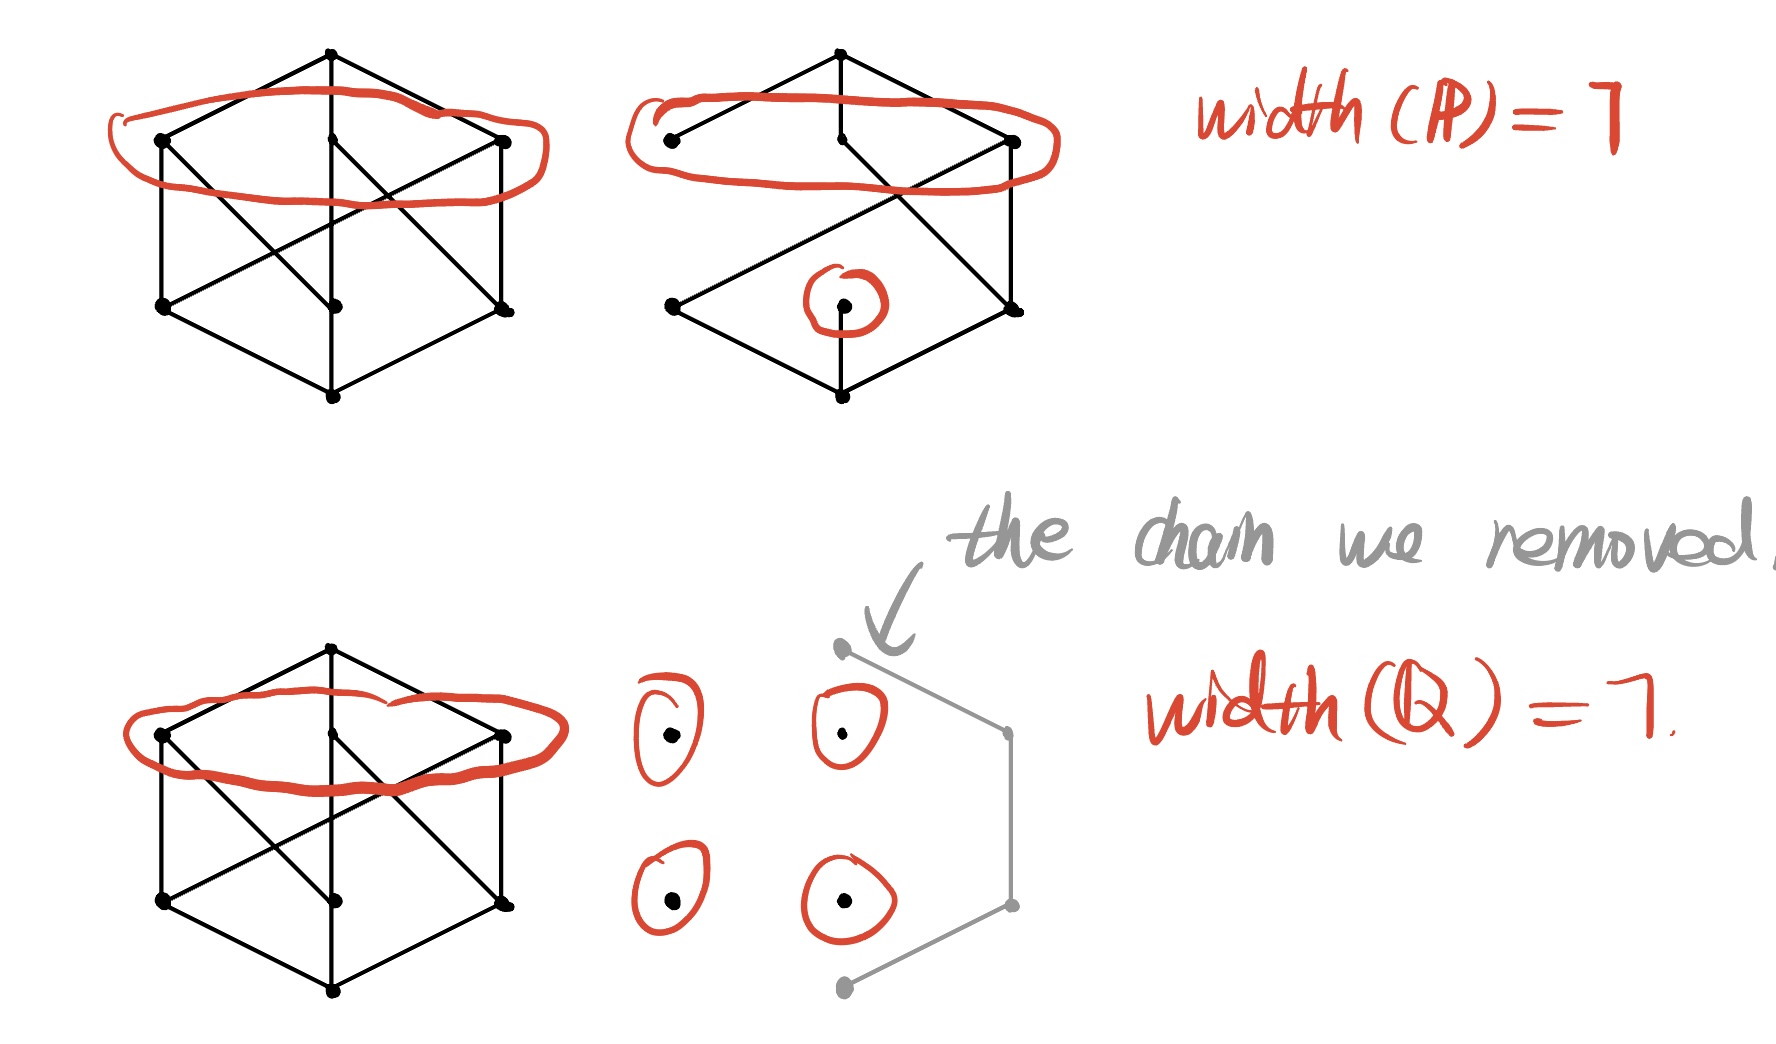
\includegraphics[scale=0.15]{Images/IMG_0308.jpg}
            \caption{A picture discription of the proof}
        \end{figure}
        Take an antichain $A=\{a_1,\cdots,a_w\} \subset X \setminus C$.\\ 
        Note, for any $a_i \in A$, $a_i$ is notbigger than $x_n$(i.e.not $x_n <_{\mathbb{P}} a_i$)else we'd contradict maximality of $C$. Define:
        \begin{itemize}
            \item $\mathbb{P}^-=\{x \in X: \exists a \in A. x \leq_{\mathbb{P}} a\}$
            \item $\mathbb{P}^+=\{x \in X: \exists a \in A. a \leq_{\mathbb{P}} x\}$
        \end{itemize}
        \begin{figure}[ht]
            \centering
            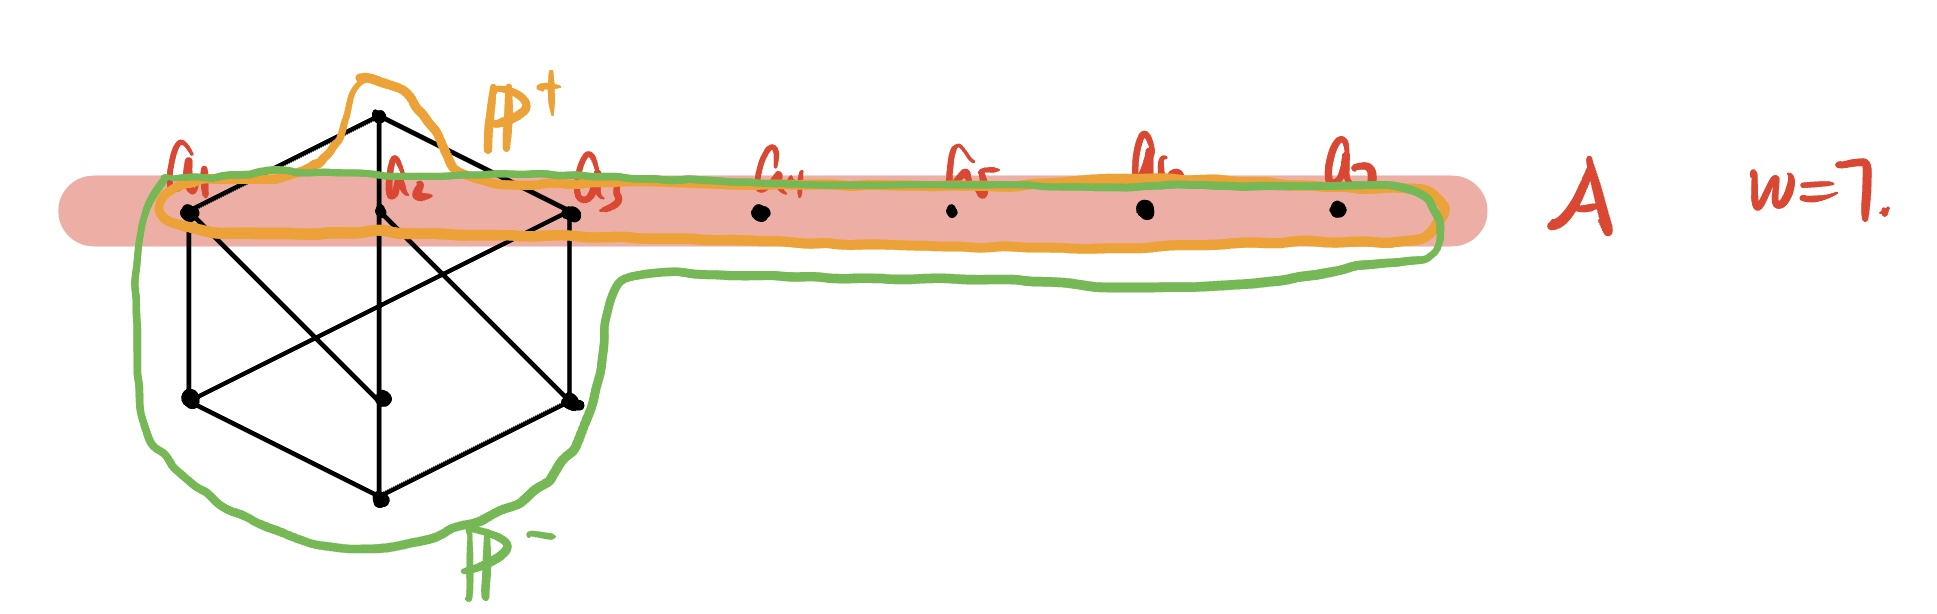
\includegraphics[scale=0.14]{Images/IMG_0309.jpg}
            \caption{A picture discription of the proof}
        \end{figure}
        Apply the induction hypothesis on $\mathbb{P}^+$ and $\mathbb{P}^-$. 
        This gives us chains $C_1^-,\cdots,C_w^-$ and $C_1^+,\cdots,C_w^+$ covering $\mathbb{P}^+$ and $\mathbb{P}^-$ respectively. 
        We may do also assume without loss of generality, $a_i \in C_i^+ \cap C_i^-$. 
        Set $C_i=C_i^+ \cap C_i^-$. This forms a family of $w$ chains cover the poset $\mathbb{P}$.
    \end{enumerate}
\end{proof}


\begin{theorem}[Erdös-Szekeres]
    Let $\{x_i: i \in [rs+1]\}$ be a family of $rs+1$ distinct real numbers. 
    There is a strictly increasing subsequence of length $r+1$ or a strictly decreasing subsequence of length $s+1$.
\end{theorem}
\begin{proof}
    Consider the poset $\mathbb{P}=(X,P)$ where $X=\{(i,x_i):i \in [re+1]\}$ and 
    $$(i,x_i) \leq_{\mathbb{P}} (j,x_j) \Longleftrightarrow i \leq j \text{ and } x_i \leq x_j$$
    If $height(\mathbb{P}) \geq r+1$, then we're done. As a maximal chain codes a strictly increasing subsequence $x_{n_k}$ of size $\geq r+1$. 
    Suppose $height(\mathbb{P}) \leq r$. Using Dilworth's theorem, can find a cover for $\mathbb{P}$ into $w=width(\mathbb{P})$ many chains $C_1,\cdots,C_w$. 
    Note that $|C_i| \leq r$, so $w \geq s+1$. Else we can cover $X$ with $\cup_{i=1}^wC_i$, which has at most $rs$ many points, contradiction. 
    It follows that there is an antichain $A=\{(n_1,x_{n_1}),\cdots,(n_{s+1},x_{n_{s+1}})\}$ where we assume that $$i<j \Longrightarrow n_i<n_j$$
    By the way we've defined $\mathbb{P}$. If $n_i<n_j$, then $x_{n_i}>x_{n_j}$. Else $(n_i,x_{n_i}) \leq_{\mathbb{P}} (n_j,x_{n_j})$, contradicting that $A$ is an antichain. 
    It follows that $x_{n_i}$ is a decreasing subsequence of size at least $s+1$.
\end{proof}
\textbf{My question}:
\begin{itemize}
    \item What is the relation between this and Bolzano-Weierstrass theorem? This looks like a finite version of Bolzano-Weierstrass theorem.
\end{itemize}

\begin{definition}
    Let $\mathbb{P}=(X,P)$ be a poset. A \textbf{linear extension} of $\mathbb{P}$ is a linear order $\mathbb{L}=(X,L)$ where $P \subset L$.i.e. a linear ordering $\leq_{\mathbb{L}}$ on $X$ with property $$a \leq_{\mathbb{P}} b \Longrightarrow a \leq_{\mathbb{L}} b$$
\end{definition}
\begin{proof}
    We do this recursively by creating a sequence of extensions $\mathbb{P}_i=(X,P-i)$ of $\mathbb{P}$, where at the terminal stage we have a linear order. 
    Suppose we're at stage $i$ and have a poset $\mathbb{P}_i$. 
    If $\mathbb{P}_i$ is not a linear order, there must be two points $a,b \in X$ that are not $\mathbb{P}_i$-comparable. 
    Construct $\mathbb{P}_{i+1}$ by setting:
    $$P_{i+1} = P_i \cup \{(a,b)\}\cup \{(x,y)\in X^2: x \leq_{\mathbb{P}_i} a \text{ and } b \leq_{\mathbb{P}_i} y\}$$
    One should confirm that $\mathbb{P}_{i+1}$ is indeed transitive. 
    Eventually this process must halt, else we'd have found an infinite sequence of pairs $(a_i,b_i)\in X^2$ that are incomparable.
\end{proof}
\textbf{Remark}:
\begin{itemize}
    \item In computer science, a topological sort or topological ordering of a directed graph is a linear ordering of its vertices.
\end{itemize}